



\section{The Monte Carlo Technique}

Monte Carlo (MC) simulations are a useful tool which provide a framework for evaluating and comparing model selection algorithms. In the context of testing and evaluating model selection algorithms, Monte Carlo simulations involve four main steps as described below. 

\subsection{Formulating the DGP} 
First, the data generating process (DGP) must be formulated. There are a number of features to consider in the DGP design which will have an impact on the success of the model selection algorithms. Of particular importance in this study is the distribution and non-centrality of the regressors. As will be explained in more detail later, the non-centrality of a particular regressor is the signal-to-noise ratio, and thus is a function of both the coefficient $\beta_{k}$ and the variance of a particular regressor. A simple example of a DGP is:
$$y_{t}=\beta_{0} + \delta y_{t-1}+\sum_{k=1}^{n}\beta_{k}x_{k,t} + \epsilon_{t},\hspace{1cm} \epsilon_{t} \sim \mathsf{IN}(0, 1)$$
$$\textbf{x}_{t} \sim \mathsf{IN_{n}}(0, \mathsf{I}) $$
for $t=1,...,T$, where $y_{0} = 0$. In practice $H+T$ draws of $\mathbf{x_{t}}$ are made and the first $H$ are the lead in to the sample for estimation.


\subsection{Running Simulations}
The second step is to perform $M$ simulations for the specified DGP, generating $M$ `replications' of the dependent variable, $\textbf{y}_{t}=(y_{1},...,y_{T})$. There are two options for drawing the regressors (excluding the lagged dependent variable $y_{t-1}$). Either new values of the regressors can be drawn for each of the $M$ simulations (stochastic regressors), or a single draw of the regressors can be used (fixed regressors). In each of the $M$ replications, a new draw of $\mathbf{\epsilon_{t}} = \epsilon_{1},...,\epsilon_{T}$ is taken.

\subsection{Formulating the GUM}
The third step is to formulate the GUM with the DGP nested within it. The GUM can include lags, nonlinearities, impulse indicators, etc. An example of a GUM associated with the DGP described above is:

$$y_{t}=\beta_{0} + \delta y_{t-1}+\sum_{k=1}^{N}\beta_{k}x_{k,t} + u_{t}  \hspace{1cm}  u_{t} \sim \mathsf{IN}[0, 1]$$

$$\mathbf{x}_{t} \sim \mathsf{IN_{N}}(0, \mathsf{I}) $$
where $N \geq n $ and $ t = 1,...,T$. To be explicit, the difference between the DGP and the GUM is that the DGP includes $n+1$ regressors while the GUM includes $N+1$ regressors. That is, $x_{1,t},...,x_{n,t}$ in the GUM are exactly the $x_{1,t},...,x_{n,t}$ in the DGP. If fixed regressors are used for $x_{1,t},...,x_{N,t}$, the GUM does not change over the $M$ simulations. If stochastic regressors are used, each of the $M$ simulations would have different draws for each of the $N$ regressors. 


 
 \subsection{Running the Algorithm}
At this point, there are $M$ sets of generated data. The final step is to run the model selection algorithm on each of these sets. The algorithm commences from the GUM, searches through the variables and returns the selected model. For each of the $M$ generated ${y_{t}}$s the algorithm selects the `best' model, eliminating some of the regressors, and providing parameter estimates for those remaining. Thus, the algorithm will produce $M$ final model estimates: one for each of the $M$ simulations. 
%(In this case of BSTS this is slightly false; the algorithm estimates distributions for the parameters. To get parameter estimates then, it is necessary to simulate or take the mean from these distributions.)






\section{Evaluating Automatic Model Selection}


Evaluating automatic model selection algorithms empirically is made difficult by the fact that the DGP is never known. This is why evaluating automatic model selection using Monte Carlo simulations is so useful. Because the DGP is precisely known, it is possible to test the accuracy with which an algorithm selects a model that is close to it. In this section, several metrics which provide a convenient means for evaluating the efficacy of model selection algorithms in Monte Carlo simulations are introduced and explained.    

\subsection{Gauge and Potency}
The gauge and potency provide measurements of the accuracy with which a model selection algorithm excludes irrelevant variables and selects relevant variables \cite{evalmodelsel}. The gauge is the proportion of the time an algorithm selects variables which are not in the DGP and the potency is the proportion of the time the algorithm selects variables which are in it. The formulas for the gauge and potency are based on another metric called the retention rate. The retention rate is the rate at which a particular regressor in the GUM is selected by the algorithm to be included in the final model. The potency is then the average retention rate across the variables which were part of the DGP. The gauge is the average retention rate across the variables which were not part of the DGP. Say there are $M$ simulations. Variables $x_{1},...,x_{n}$ are in the DGP, making these the relevant variables. Variables $x_{n+1},...,x_{N}$ are not in the DGP, making these the irrelevant variables. Let $\beta_{1},...,\beta_{N}$ be the true parameter values, so that $\beta_{n+1},...,\beta_{N}=0$. Let $\widetilde\beta_{k,i}$ be the estimated coefficient on variable $x_{k}$ in simulation $i$  for each of the $N$ variables following model selection. If a particular variable is not selected in a simulation, $\widetilde\beta_{k,i}=0$. Let $1(\cdot)$ be an indicator variable with $1(\cdot)=1$ if $x_{k}$ is selected (so $\widetilde\beta_{k}\neq 0$) and $1(\cdot) = 0$ if $x_{k}$ is not selected (so $\widetilde\beta_{k}=0$). The retention rate, potency and gauge are defined as: 
\begin{align*}
&\mathrm{retention\ rate}:   \widetilde p_{k} = \frac{1}{M} \sum_{i=1}^{M}1(\beta_{k,i} \neq 0)\\
&\mathrm{potency} = \frac{1}{n} \sum_{k=1}^{n} \widetilde p_{k}\\
&\mathrm{gauge} = \frac{1}{N-n} \sum_{k=n+1}^{N} \widetilde p_{k}
\end{align*}
Note that usually the intercept is not included in the potency and gauge calculations as it is almost always selected and is often forced. Similarly depending on the nature the DGP the lagged dependent variable is often excluded as well. 






%Retention rate: $$\[\frac{1}{1000}\]$$


\subsection{Mean Squared Errors}



The mean squared errors (MSEs) provide a measure for the accuracy of the parameter estimates. Here, a distinction is made between conditional and unconditional MSEs. If there are $M$ simulations, the conditional MSE for variable $x_{k}$ is calculated as:

$$ \textrm{CMSE}_{k} = \frac{\sum_{i=1}^{M}[(\widetilde\beta_{k,i} - \beta_{k})^{2} \cdot 1(\widetilde\beta_{k,i} \neq 0)]}{\sum_{i=1}^{M}1(\widetilde\beta_{k,i} \neq 0)},\-\-\-\-\ (\beta_{k,i}^{2} \textrm{ when  } \sum_{i=1}^{M}(1(\widetilde\beta_{k,i} \neq 0)=0)$$

where $\widetilde\beta_{k,i}$ is the estimated parameter if $x_{k}$ is selected. The unconditional MSE is defined as:

$$ \textrm{UMSE}_{k} = \frac{1}{M}\sum_{i=1}^{M}(\widetilde\beta_{k,i} - \beta_{k})^{2}, \; \forall \; k$$
If $x_{k}$ is not selected, then $\widetilde\beta_{k,i} = 0$. In this thesis the square root of the conditional mean squared errors denoted RCMSE is reported. Whereas the $\textrm{CMSE}_{k}$ averages across simulations in which a particular $x_{k}$ is selected, $\textrm{UMSE}_{k}$ takes the average across every simulation.  The UMSE is a measure which many authors report, however in this study it is not reported because the CMSE, when interpreted alongside the gauge and potency, is much more informative. For example, say that a retention rate of a particular irrelevant variable $x_{k}$ is 0.01; that is, it is selected in 10 of 1000 simulations. Then, irrespective of what the parameter estimates in those 10 cases were, the UMSE is going to close to be 0. On the other hand, the CMSE provides a measure of how close (or far) the estimates are to the true parameter ($\beta_{k} = 0$) in those 10 cases and can actually be quite large. Similarly, consider a relevant variable $x_{j}$ which has a potency of 0.6, and is not selected in 400 of 1000 simulations. The UMSE for $x_{j}$, of course, will include the estimates from those 400 simulations where $x_{j}$ is not selected, and $\widetilde\beta_{j,i}=0$. For a relevant variable which has a relatively low potency then, the UMSE can end up being quite large, and says little about the accuracy of the parameter estimates themselves. The CMSE on the other hand provides a measure of how effective an algorithm is at actually estimating parameters, which taken alongside the gauge and potency, is much more useful. Additionally, in empirical research only the conditional selected model is known meaning that the properties of selected models are more useful when evaluating selection algorithms. While UMSEs are not reported in this study, they are available upon request. 


\subsection{A Note on Statistical Size}

At first glance, the `size' of each algorithm might seem like an informative metric to include. In statistics, size refers to the probability of a Type 1 error, namely that the null hypothesis is rejected when it is true. In the context of model selection algorithms, size is then the probability that the DGP is not selected, which in simulations corresponds to the proportion of the time that either a relevant variable is excluded or a irrelevant variable is included in the selected model. Under the null that $\beta_{k} = 0$ the probability of excluding an irrelevant variable is $(1-\alpha)$. Then, if there are $N-n$ irrelevant variables, the probability that they are all excluded is $(1-\alpha)^{N-n}$. The probability of retaining a single irrelevant variable is then $ 1 - (1-\alpha)^{N-n}$ which could be very high, especially if there are many irrelevant variables. It is for this reason that the size of each procedure is not reported. It seems sensible to accept that while model selection may not always select the precisely correct DGP, there is immense value in excluding `garbage', a fact which is largely overlooked when statistical size is used. Note that statistical size is very dependent on the number of irrelevant variables $N-n$. However since the GUM includes many variables to ensure that nothing important is missed, it will usually be the case that $N-n$ is sufficiently large to result in a high statistical size.




\section{The Benchmark}

Comparing the gauge, potency and RCMSE across different algorithms tells an interesting story in itself. Another interesting and related story however, is how these results compare to the `benchmark' or `best case scenario'. In the context of model selection, the `best case scenario' means doing model selection under the conditions which offer the `best chance' for an algorithm to successful identify the DGP. Identifying the benchmark allows the results of model selection to be qualified. What the optimal conditions are depends on the DGP specification, and specifically whether or not the regressors are orthogonal or not. These two cases are considered in turn.

\subsection{Orthogonal Regressors}

Consider first the case of orthogonal regressors, and specifically consider the following DGP:

$$y_{t}=\beta_{0} + \delta y_{t-1}+\sum_{k=1}^{n}\beta_{k}x_{k,t} + \epsilon_{t}, \hspace{.5cm} \epsilon_{t} \sim \mathsf{IN}(0, 1) $$
$$\mathbf{x}_{t} \sim \mathsf{IN_{k}}(0, I) $$
for $t=1,...,T$. Now suppose the researcher (magically) knew precisely which variables were in the DGP and estimated the following model:

$$y_{t}=\beta_{0} + \delta y_{t-1}+\sum_{k=1}^{n}\beta_{k}x_{k,t} + u_{t} $$
This is the `best case scenario' for finding the DGP; every relevant variable is included in the model being estimated with no irrelevant variables that could be mistakenly selected. In real life, however, it would be impossible to know that modelling was in fact commencing from the DGP and a good econometrician naturally would be interested in conducting inference to determine which variables, from a statistical perspective, were significant. This would generally be done via t-statistics, with high $p$-values leading the researcher to conclude that those variables were insignificant. The results from conducting this process which is referred to as selection from the DGP are therefore the benchmark when the regressors are orthogonal. 

This idea is captured in a model selection technique called the 1-cut approach. Consider the following GUM, with $N<<T$:

$$y_{t} = \beta_{0} + \sum_{k=1}^{N}\beta_{k}x_{k,t} + u_{t}$$

Because $N<<T$, the GUM can be estimated directly, resulting in coefficient estimates and standard errors for $\beta_{1},...,\beta_{N}$. Then $t$-statistics are computed and ordered as follows: 
$$t_{(1)}^{2} \geq t_{(2)}^{2} \geq ... \geq  t_{(N)}^{2}$$

Variables with $t_{k}^{2} \geq c_{\alpha}^{2}$ are retained. Thus only a single decision is required to select variables; there is no `data mining' or repeated testing. 

The 1-cut approach embodies the approach that a researcher may and usually will undertake in practice (although it is not explicitly referred to as model selection). Therefore, the potency and RCMSE results from the 1-cut approach on the DGP are reported alongside the potency, retention rate and RCMSE results from the three algorithms. This provides some context for the results from the model selection algorithms. For example, if a particular set of simulations shows that a model selection algorithm has a potency of 0.4 and selects relevant variables 40\% of the time, critics may be inclined to dismiss the algorithm as ineffective and inaccurate. This is not a valid criticism, however, if when estimating from the DGP itself, relevant variables are deemed insignificant by their $t$-tests (or equivalently, not selected by 1-cut) a similar proportion of the time. To re-iterate, if in the `best case' scenario a relevant variable is deemed irrelevant or insignificant, it should not come as surprise or indeed be considered a `drawback' if this variable is not selected by a model selection algorithm, amongst many other variables. Model selection algorithms should not lose credibility if they are unsuccessful at finding `significant variables' which are not even `significant' when the model is estimated from the DGP. It should also be noted that even when the regressors are orthogonal, there will be some amount of correlation between the regressors for any given sample, meaning that algorithms have the potential to outperform the 1-cut approach, which is explained in more detail below.


 

\subsection{Correlated Regressors}

When the regressors are correlated, the 1-cut approach is not valid. The best hope a researcher would have at finding variables which matter in this case would be to use a model selection algorithm which is equipped to deal with correlation (which Autometrics, the Lasso, and BSTS all claim to be) on the DGP itself. Because each of the algorithms employ different approaches to model selection, and the question over which one is the `best' is subjective, the benchmark for a particular algorithm are the results from using that algorithm to select from the DGP.  To make this more formal, consider the following DGP:


$$y_{t}=\beta_{0} + \delta y_{t-1}+\beta_{1}x_{1,t}+\beta_{2}x_{2,t}+ \beta_{3}x_{3,t}+ \beta_{4}x_{4,t}+ \beta_{5}x_{5,t} + \epsilon_{t}$$
$$\centerline{$\epsilon_{t} \sim $ IN[0,1] }$$
 $$\centerline{$\textbf{x}_{t} \sim $ IN\textsubscript{N}[0,$\Omega$]}$$
with $\omega_{kk} = 1$ and $\omega_{jk} = 0.9$ for $j \neq k $ for $t=1,...,T$. Now suppose the researcher knew which variables were relevant and used the following GUM:

$$y_{t}=\beta_{0} + \delta y_{t-1}+\beta_{1}x_{1,t}+\beta_{2}x_{2,t}+ \beta_{3}x_{3,t}+ \beta_{4}x_{4,t}+ \beta_{5}x_{5,t} + u_{t}$$
The benchmark for an algorithm searching through a much larger GUM would be the potency and RCMSE results from commencing from the above GUM, which is the true DGP. When regressors are correlated, it is precisely these conditions which allow the algorithm the best chance at selecting the correct model. 

%Is benchmark for CMSE estimating directly??? Ask Jennie

%Discussion of why theoretical retention probabilies are reported: ie. because they only apply to 1-cut so why are the relevant for model selection? Because it turns out Autometrics results are CLOSE to the theoretical properties behind the 1-cut - which means in an empirical setting we can, i.e., adjust alpha and have an idea of the results we are getting - that is, how many irrelevant variables and what the retention rates would be! This is related the the above


\section{Interpreting the Results}

The results from the Monte Carlo simulations that are presented in the next section provide insight into three questions: (1) how algorithms perform relative to one another given a particular correlation structure, (2) how algorithms perform relative to their respective benchmarks and (3) more broadly how the results of empirical model selection using Autometrics, the Lasso and BSTS can be interpreted. The next section details how the gauge, potency, retention rates, RCMSE and benchmark results provide insight into these questions.

\subsection{Algorithm vs. Algorithm}

The gauge, potency and RCMSE from selection from the GUM make it easy to compare the algorithm's performance within a particular correlation structure.  High potencies, low gauges and low RCMSEs are all desirable in the MC simulations. 

\subsection{Algorithm vs. Benchmark}

Evaluating the algorithm's results against their benchmark by comparing the potencies, retention rates and RCMSEs in each case is straightforward. If the results from model selection are similar to the benchmark then the algorithm is performing as well as could optimistically be expected. A productive framework for thinking about this is considering the costs of inference and the costs of search. Costs of inference are inevitable even for a modeller who commenced from the DGP but (as is always the case in economics) did not know if the specification was correct and thus conducted inference. Similarly, there are obviously costs of inference when using automatic model selection on a GUM of any size. These costs can be measured with the RCMSE values. Costs of search are the additional costs, and are the result of commencing from a more general model. The difference between the RCMSE when commencing from the GUM and the RCMSE when commencing from the DGP (either using 1-cut or using model selection directly on the DGP) measures the costs of search for a particular model selection algorithm. Thus, the benchmark DGP results reported in the results tables are useful because they provide context for the cost of inference when performing model selection (via the RCMSEs), and also provide a measure of the cost of model selection (via the RCMSE differences).   
%Look at David's book for more info on costs of inference
\subsection{Simulation Results vs. Empirical Model Selection}
MC simulations provide lots of interesting results but they are just that: simulations. A valid question is what MC results say about model selection empirically. The difficulty with MC simulations is that their results are generally limited to the specified DGP. That is, the potency and gauge measures for a particular set of simulations would only be directly relevant in a real world situation where the DGP has the exact same specification as in the MC simulation. As has been discussed, this is an impossible problem. A method is therefore required, which allows the results of MC simulations to be `mapped' to empirical model selection. This is mostly easily done with the use of the non-centrality parameter.

Intuitively, regressors which are `highly significant' should be `picked up' more frequently than those which are less significant. A measure which provides a useful interpretation of the `significance' of a variable $x_{k}$ is the non-centrality of $x_{k}$, denoted $\psi_{k}$. The non-centrality is the `signal-to-noise' ratio, where the signal is the value of the parameter $\beta_{k}$ and the noise is $\sigma_{\beta_{k}}$. The non-centrality is therefore just the expectation of the t-statistic for variable $x_{k}$:
%10 See McQuarrie and Tsai (1998) for the importance of ?signal-to-noise? ratio as a determinant of MSA performance for IC algorithms. 
$$t_{\widehat{\beta}_{k}}=\frac{\widehat{\beta}_{k}}{\widehat{\sigma}_{\widehat{\beta}_{k}}} \simeq \frac{\widehat{\beta}_{k}}{\sigma_{\widehat{\beta}_{k}}} \sim \mathsf{N} \Bigg[\frac{\beta_{k}}{\sigma_{\widehat{\beta}_{k}}}, 1 \Bigg] = \mathsf{N} \big[\psi_{k}, 1 \big] $$
Therefore, the formula for $\psi_{k}$ is given by:

$$\psi_{k} = \frac{\beta_{k}}{\sigma_{\widehat{\beta}_{k}}}$$
The above formula makes explicit that relationship between $\psi_{k}$, the coefficient $\beta_{k}$ and the variance $\sigma_{\widehat{\beta}_{k}}^{2}$. The non-centrality is useful in understanding the relationship between the specification of the DGP and the potency or retention rates of particular variables. Consider, as discussed earlier, estimating a model directly from the DGP, and obtaining the $t$-statistics for each of the relevant variables. Because the DGP is known, it is possible to derive the distribution of the $t$-statistics and as the above formulas suggest, the non-centrality of a variable characterizes this distribution. Knowing the $t$-statistic distribution means it is possible to determine the probability that a variable is deemed significant, or more formally, the probability that the null $H_{0}: \beta_{k} = 0$ is rejected for a given significance level $\alpha$. This probability is called the theoretical retention probability, and is calculated from:

$$ \mathsf{P}_{\alpha} = \Pr( \hspace{0.1cm}|t_{k}| \hspace{0.1cm} \geq \hspace{0.1cm} c_{\alpha} \hspace{0.1cm} | \hspace{0.1cm}\psi_{k}\hspace{0.1cm}) = \Phi({c_{\alpha}-\psi_{k}})$$
where $\Phi(x)$ denotes the integral of the normal density. It is possible to calculate the theoretical retention probability for every non-centrality and significance level. This is important because as it turns out certain algorithms have retention rates which are in line with the calculated theoretical retention probabilities. 

%To better understand the relationship between the non-centrality and the theoretical retention probability, it is useful to consider what the distribution of the t-statistics looks like under the null, and for varying values of $psi_{k}$. Under the null, t-statistics have a distribution which is approximately N(0,1), and for example, consider the significance level $\alpha = 0.01$ which corresponds to the $c_{\alpha}=2.67$. The critical region is shaded in the graph below.
%insert density graph

%Now consider a variable which has a non-centrality $\psi_{k}=2$. The distribution of its t-statistic can be approximated by N(2,0). Now, the null will be rejected if the t-statistic is greater than $c_{\alpha} = 2.67$. As can be seen from the graph, the probability of drawing values greater than 2.67 is (....). This is the theoretical retention probability discussed above.

%Theoretical properties are straightforward to calculate under the 1-cut approach with orthogonal variables. Under the null $H_{0}:\beta_{k}=0$, the theoretical false null rejection probability of a particular irrelevant variable is $\alpha$, and the theoretical false null rejections across all irrelevant variables is $N\alpha$. Therefore, in the 1-cut approach, false retentions can be controlled for by setting tight significance levels. If there are 1000 irrelevant variables, setting $\alpha = 0.001$ means only 1 irrelevant variable will be falsely retained.

%Discussion of why we include it! i.e. why when we move empirical results it helps us interpret results


%To reiterate, the theoretical retention probability is the probability of correctly rejecting the null $H_{0}: \beta_{k} = 0$ based on a single t-statistic, when estimation does not involve model selection and commences from the LDGP. This is useful because potency measures from the simulations demonstrate that the potency of certain algorithms are close to the measure of the theoretical retention probability. This allows us, in an empirical setting for an given significance level $\alpha$ to derive inferences about the selected model. For example, if we chose alpha to be 0.01, then we know that for any variable with a non-centrality of 6 , there is a 99 percent chance that it has been selected. On the other side, we know that a variable with a low non-centrality, say 2, there is a 65 percent chance that it has been selected. There is no direct calculation of this sort to determine, using the selection algorithms directly, which allows to draw similar inference. That is, you can use the Lasso on any data set, but since you do not know the true parameters, it is difficult to understand or draw any inference as to what the properties or conditions of the variables that were selected actually are. But if there is a relation in the simulations between TRR and the potency, it IS possible to draw conclusions about the selected variables.





%A related question is what affects the gauge. Because irrelevant variables (obviously) are not in the DGP, there is nothing in the specification of the DGP that should affect the measure of the gauge. In the specification of the GUM, however, orthogonality or otherwise between regressors has an impact on the gauge (???) is this true???. A reminder that the gauge is the proportion of time irrelevant variables are selected by the algorithm. Thus, the expected gauge would be derived from the properties of the algorithms themselves. Indeed, in Autometrics, the gauge can be controlled directly by the signficance level $\alpha$. The theory behind this comes from estimating a model (when N<T) directly using OLS. The distribution of the t-statistics for relevant variables is then known - N(0,1). So by design, the t-statistic will lie in the critical region $(1-\alpha$ percent of the time, and $\alpha$ percent of the time, the t-statistic will lie outside of the critical region and the null will be rejected. For individual t-tests, then, a small value of $\alpha$ reduces the probability of falsely rejecting the null. Across all N irrelevant variables then, the number of falsely retained variables is $N\alpha$. Thus setting $\alpha$ very small controls for spurious regressors to be included in the selected model.

%Obviously Autometrics involves multi-path search and therefore the distribution of the t-statistics is not quite as simple. In Autometrics, the signficance level, $\alpha$ is set, however, and it corresponds to [....] as outlined in early sections. Multiple simulations have show that, however, the gauge is very close to the set significance level $\alpha$. 

%For the LASSO it is less clear theoretically how to control for the gauge. The only `tool' available to control the results is in the tuning parameter, however simulations indicate that this does not have a drastic impact on the results. In general, however, a higher tuning parameter would result in more coefficients being set to zero, thus impacting the gauge. The Lasso theory is fuzzier: while there are various ways to choose the tuning parameter, there is no way direct, proven method to control for selecting irrelevant variables. Even testing our various tuning parameters, the tuning parameter seems to have little effect on the measurements of gauge in the simulations. 

%Work done by Hendry, Castle, Doornik, etc., has shown, however, that despite multiple-path seach, Autometrics performs similarly to the one-cut approach, and that the theoretical properties hold even as N>T. Clearly, the 1-cut is only valid when there are fewer regressors than observations, which is a clear limitation in model selection. However, previous work has demonstrated that Autometrics continues to perform as N increases. For Autometrics, therefor, the gauge can be controlled by setting tight signficance levels. 


%In BSTS, you can indirectly adjust for the gauge by setting the expected model size via the prior that is set by the researcher. Again, this is fuzzy and in simulations does not seem like a surefire way for insuring that irrelevant variables are excluded from the final model.

%\textbf{But hold on one second: N>T???}

%\textbf{Orthogonal vs Non-orthogonal}


%\textbf{Costs of Search and Inference}
 
%\textbf{Lasso}



%\textbf{BSTS}


\section{Experimental design}

The experimental design consists of three separate sets of experiments. In the first, the regressors are all orthogonal, in the second there is correlation between the relevant regressors, and in the third there is correlation between all regressors. In all three sets of experiments the algorithm settings remain constant; these settings are outlined in the next section. Furthermore, the DGPs and more specifically the values of the non-centralities $\psi_{k}$ are chosen in such a way that the results are comparable across the three separate sets of experiments. In the following sections, the DGPs and GUMs are described and the results are presented for each of the three sets of experiments. The final section provides a summary of results.

\subsection{Algorithm Settings}

As discussed in Chapter 2, there are a number of decisions that must be made when applying the algorithms. The following table outlines the settings for the three algorithms compared, as well as the relevant software that was used for the simulations.

%TABLE for algorithm settings 
\begin{table}[h]
\centering
\begin{tabular}{p{2cm}| p{3cm}| p{3cm}| p{3.5cm}}

\textbf{Algorithm}& \textbf{Software/Relevant package} & \textbf{User input} & \textbf{Comment}  \\
\hline
\small{Autometrics} & \small{OxMetrics version 7.00}&\small{$\alpha = 0.01$} & \small{All other defaults used, as described in Table \ref{tab:algsettings} } \\

\hline
\small{Lasso} & \small{R version 3.2.3, glmnet package} &\small{$\lambda$ chosen by 10-fold cross validation}& \small{K-fold cross validation built into glmnet}\\
& && \\
\hline
\small{BSTS} &\small{R version 3.2.3, bsts package} &\small{$R^{2} = 0.5$, and $v=0.01$} & \small{All default priors used} \\
\end{tabular}
\caption{Algorithm settings}
\label{AlgoSettings}
\end{table}
An additional setting for BSTS was the decision to consider variables with posterior inclusion probability greater than $0.15$ as selected. While this seems low, it was rare to observe posterior inclusion probabilities greater than $0.2$. 

%END OF TABLE for algorithm settings




\subsection{Orthogonal Regressors}

The first set of experiments considers cases where the regressors, with the exception of the lagged dependent variable, are mutually orthogonal. There are three different DGPs considered, which vary according to the coefficients $\beta_{1},...,\beta_{5}$. The values of these coefficients affect the non-centralities $\psi$, which is a more interpretable characterization. The $\beta_{0}$ and $\delta$ coefficients are the same across all experiments, with $\beta_{0}=1$ and $\delta= 0.5$.  Each of these DGPs is nested in two separate GUMs: one with the total number of regressors $N$, excluding the lagged dependent variable (LDV),  as $N=80$ and the second with $N=120$. In all experiments, $T=100$. Thus, there are six separate experiments performed for the case of orthogonal regressors. In all experiments, fixed regressors were used. Note that in practice, in any given sample there will be degree of correlation between the simulated $x_{1},...,x_{N}$, and that when  $N>>T$ orthogonality is in fact impossible. Nevertheless, variables can be generated so that correlation between them is small. Let $\textbf{x}_{t}'=(x_{1,t},...,x_{N,t})$. The DGPs take the following form: 
$$y_{t}=\beta_{0} + \delta y_{t-1}+\beta_{1}x_{1,t}+\beta_{2}x_{2,t}+ \beta_{3}x_{3,t}+ \beta_{4}x_{4,t}+ \beta_{5}x_{5,t} + \epsilon_{t}$$
$$\epsilon_{t} \sim \mathsf{IN}[0,1] $$
$$\textbf{x}_{t}=0.5\textbf{x}_{t-1}+\textbf{v}_{t}, \textbf{v}_{t} \sim \mathsf{IN}_{N}[0,\Omega]$$
with the persistence parameter $\rho = 0.5$, $\omega_{kk} = 1-\rho^{2} = 0.75$ and $\omega_{jk} = 0 $ for $j \neq k$. While this may seem like an arbitrary choice for the variance-covariance matrix $\Omega$, it has been chosen because the resulting non-centralities are integers and in line with previous studies. Note that the results that follow break down as $\rho\rightarrow 1$, but since $\rho=0.5$ here it is not a issue. Table \ref{DGPspec123} describes the three DGPs considered in this set of experiments, and gives the theoretical retention probabilities $ \mathsf{P}_{0.01}$. Because the regressors are orthogonal in this set of experiments, the benchmark is model selection from the DGP via the 1-cut approach.  

%TABLE DGPs of experiments including orthogonal variables
\begin{table}[h]
\centering
%\begin{tabular}{l|l|l|l|l|l|l|l}
\begin{tabular}{r |r |r |r |r |r |r}

&  &$x_{1}$ &$x_{2}$ &$x_{3}$ &  $x_{4}$ & $x_{5}$  \\
\hline
\textbf{DGP 1} & $\beta_{k}$  & 0.6 &0.6 &0.6 &  0.6 & 0.6 \\

 	& $\psi$  &6 &6 &6 &6 &6 \\
 
   & $ \mathsf{P}_{0.01}$  & 0.999 & 0.999 & 0.999 & 0.999 & 0.999 \\
\hline
\textbf{DGP 2} & $\beta_{k}$ &  0.2 &0.2 &0.2 &  0.2 & 0.2 \\

 	& $\psi$  &2 &2 &2 &2 &2 \\
       & $ \mathsf{P}_{0.01}$ & 0.266 & 0.266 & 0.266 & 0.266 & 0.266 \\
\hline
\textbf{DGP 3} & $\beta_{k}$  & 0.2 &0.3 &0.4 &  0.5 & 0.6 \\

 	& $\psi$  &2 &3 &4 &5 &6 \\
       & $ \mathsf{P}_{0.01}$ & 0.266 & 0.645 & 0.914 & 0.990 & 0.999 \\
    
\end{tabular}
\caption{DGP specification for experiments with orthogonal $x_{k}$s}
\label{DGPspec123}
\end{table}


%END OF TABLE DGPs of experiments including orthogonal variables

Each DGP is nested in two separate GUMs, one with $N=80$, and one with $N=120$. These two GUMs take the following form:
$$y_{t}=\beta_{0} + \delta y_{t-1}+\sum_{k=1}^{N}\beta_{k}x_{k,t} + u_{t}$$
Tables \ref{DGP1GP} and \ref{DGP2GP} report the gauge and potency for the DGP 1 and DGP 2 respectively, while Table \ref{DGP1CMSE} and Table \ref{DGP2CMSE} report their RCMSE results. The lowest gauge, highest potency and lowest RCMSE are in bold. Figures \ref{RCMSECase1a} and \ref{fig:RCMSECase2a} graph the RCMSE results. Tables \ref{DGP3GP}-\ref{DGP3RR} report the results for DGP 3 and Figures \ref{fig:CMSEDGP3a} and \ref{fig:RCMSECase2a} graph these results. There are varying non-centralities in DGP 3 which is why Table \ref{DGP3RR} reports the retention rates and the theoretical retention probabilities for each individual relevant regressor.  
\\
% Table generated by Excel2LaTeX from sheet 'GPChartCase1-2'
\begin{table}[htbp]
  \centering
 
    \begin{tabular}{r|r|r|r|r}

         & \multicolumn{2}{|c|}{\textbf{$N=80$}} & \multicolumn{2}{|c}{\textbf{$N=120$}} \\
            & Potency           & Gauge           & Potency            & Gauge           \\
          \hline
    \textbf{Autometrics} & 0.994 & 0.013 & 0.991 & 0.013 \\
    \textbf{Lasso} & \textbf{1.000} & 0.216 & \textbf{0.997} & 0.174 \\
    \textbf{BSTS} & 0.715 & \textbf{0.001} & 0.757 & \textbf{0.000} \\
    \hline
    \textbf{DGP} & 0.999 & N/A   & 0.999 & N/A \\

    \end{tabular}%     
 
  \caption{Gauge and potency for DGP 1} 
   \label{DGP1GP}%
\end{table}%


% Table generated by Excel2LaTeX from sheet 'GPChart3-4'
\begin{table}[htbp]
  \centering

    \begin{tabular}{r|r|r|r|r}

         & \multicolumn{2}{|c|}{\textbf{$N=80$}} & \multicolumn{2}{|c}{\textbf{$N=120$}} \\
            & Potency           & Gauge           & Potency            & Gauge           \\
          \hline
    \textbf{Autometrics} & 0.320 & 0.029 & 0.263 & 0.029 \\
    \textbf{Lasso} & \textbf{0.526} & 0.146 & \textbf{0.428} & 0.125 \\
    \textbf{BSTS} & 0.022 & \textbf{0.001} & 0.023 & \textbf{0.001} \\
    \hline
    \textbf{DGP} & 0.278 & N/A   & 0.278 & N/A \\

    \end{tabular}%
      \caption{Gauge and potency for DGP 2}
  \label{DGP2GP}%
\end{table}%





% Table generated by Excel2LaTeX from sheet 'CMSEChartCase1-2'
\begin{table}[htbp]
  \centering

    \begin{tabular}{r|r|rrrrrr}

          &       & $y_{t-1}$ & $x_{1}$ & $x_{2}$ & $x_{3}$ & $x_{4}$ & $x_{5}$ \\

          & $\delta/\beta_{k}$ & 0.5   & 0.6   & 0.6   & 0.6   & 0.6   & 0.6 \\
          \hline
          \hline
$\bm{N=80}$ & \textbf{Autometrics} & \textbf{0.057} & \textbf{0.112} & \textbf{0.127} & \textbf{0.099} & \textbf{0.105} & \textbf{0.111} \\
    \textbf{} & \textbf{Lasso} & 0.085 & 0.201 & 0.196 & 0.183 & 0.173 & 0.201 \\
    \textbf{} & \textbf{BSTS} & 0.082 & 0.274 & 0.259 & 0.232 & 0.235 & 0.238 \\
    \hline
    \textbf{} & \textbf{DGP} & 0.055 & 0.097 & 0.102 & 0.110 & 0.105 & 0.108 \\
    \hline
    \hline
    $\bm{N=120}$ & \textbf{Autometrics} & \textbf{0.068} & \textbf{0.106} & \textbf{0.113} & \textbf{0.129} & \textbf{0.121} & \textbf{0.107 }\\
    \textbf{} & \textbf{Lasso} & 0.124 & 0.165 & 0.204 & 0.285 & 0.215 & 0.239 \\
    \textbf{} & \textbf{BSTS} & 0.105 & 0.186 & 0.262 & 0.273 & 0.241 & 0.211 \\
    \hline
    \textbf{} & \textbf{DGP} & 0.055 & 0.097 & 0.102 & 0.110 & 0.105 & 0.108 \\
        

    \end{tabular}%
      \caption{RCMSE for DGP 1}
  \label{DGP1CMSE}%
\end{table}%



% Table generated by Excel2LaTeX from sheet 'CMSEChartCase3-4'
\begin{table}[htbp]
  \centering
   \begin{tabular}{r|r|rrrrrr}

          &       & $y_{t-1}$ & $x_{1}$ & $x_{2}$ & $x_{3}$ & $x_{4}$ & $x_{5}$ \\
          & $\delta/\beta$ & 0.5   & 0.2   & 0.2   & 0.2 & 0.2   & 0.2 \\
             \hline
          \hline
    $\bm{N=80}$ & \textbf{Autometrics} & \textbf{0.120} & 0.164 & 0.221 & 0.124 & 0.142 & 0.151 \\
    \textbf{} & \textbf{Lasso} & 0.218 & \textbf{0.129} & 0.137 & 0.128 & \textbf{0.127} & \textbf{0.133} \\
    \textbf{} & \textbf{BSTS} & 0.153 & 0.216 & \textbf{0.125} & \textbf{0.119} & 0.141 & 0.221 \\
    \hline
    \textbf{} & \textbf{DGP} & 0.091 & 0.119 & 0.126 & 0.161 & 0.146 & 0.157 \\
    \hline
    \hline
    $\bm{N=120} $& \textbf{Autometrics} & \textbf{0.139} & 0.140 & 0.162 & 0.210 & 0.180 & 0.146 \\
    \textbf{} & \textbf{Lasso} & 0.258 & \textbf{0.123} & \textbf{0.130} & 0.139 & \textbf{0.131} & 0.132 \\
    \textbf{} & \textbf{BSTS} & 0.191 & 0.182 & 0.180 & \textbf{0.084} & 0.159 & \textbf{0.131} \\
    \hline
    \textbf{} & \textbf{DGP} & 0.091 & 0.119 & 0.126 & 0.161 & 0.146 & 0.157 \\

    \end{tabular}%
      \caption{RCMSE for DGP 2}
  \label{DGP2CMSE}%
\end{table}%

% Table generated by Excel2LaTeX from sheet 'GaugePotencyDGP3'
\begin{table}[htbp]
  \centering

    \begin{tabular}{r|r|r|r|r}

         & \multicolumn{2}{|c|}{\textbf{$N=80$}} & \multicolumn{2}{|c}{\textbf{$N=120$}} \\
            & Potency           & Gauge           & Potency            & Gauge           \\
          \hline
    \textbf{Autometrics} & 0.712 & 0.018 & 0.708 & 0.021 \\
    \textbf{Lasso} & \textbf{0.877} & 0.179 & \textbf{0.835} & 0.146 \\
    \textbf{BSTS} & 0.361 & \textbf{0.001} & 0.334 & \textbf{0.001} \\
    \hline
    \textbf{DGP} & 0.766 & N/A   & 0.766 & N/A \\

    \end{tabular}%
      \caption{Gauge and potency for DGP 3}
  \label{DGP3GP}%
\end{table}%



% Table generated by Excel2LaTeX from sheet 'RetRatesChartDGP3'
\begin{table}[htbp]
  \centering

    \begin{tabular}{r|r|rrrrr}

          & \boldmath{}\textbf{$\psi$}\unboldmath{} & 2     & 3     & 4     & 5     & 6 \\
        

          & \textbf{$\mathsf{P}_{0.01}$} & 0.266 & 0.645 & 0.914 & 0.990 & 0.999 \\
            \hline
          \hline
   $ \bm{N=80}$ & \textbf{Autometrics} & 0.216 & 0.414 & 0.948 & 0.989 & 0.995 \\
    \textbf{} & \textbf{Lasso} & \textbf{0.552 }& \textbf{0.869} & \textbf{0.974} & \textbf{0.995 }& \textbf{0.996} \\
    \textbf{} & \textbf{BSTS} & 0.003 & 0.136 & 0.325 & 0.562 & 0.781 \\
    \hline
    \textbf{} & \textbf{DGP} & 0.331 & 0.672 & 0.847 & 0.982 & 1.000 \\
    \hline
    \hline
   $ \bm{N=120}$ & \textbf{Autometrics} & 0.367 & 0.573 & 0.655 & 0.953 & 0.992 \\
    \textbf{} & \textbf{Lasso} & \textbf{0.669} & \textbf{0.779} & \textbf{0.740} & \textbf{0.989} & \textbf{0.997} \\
    \textbf{} & \textbf{BSTS} & 0.059 & 0.036 & 0.092 & 0.602 & 0.880 \\
    \hline
    \textbf{} & \textbf{DGP} & 0.331 & 0.672 & 0.847 & 0.982 & 1.000 \\

    \end{tabular}%
      \caption{Retention rates for DGP 3}
  \label{DGP3RR}%
\end{table}%
% Table generated by Excel2LaTeX from sheet 'CMSEChartDGP3'
\begin{table}[htbp]
  \centering

   \begin{tabular}{r|r|rrrrrr}

          &       & $y_{t-1}$ & $x_{1}$ & $x_{2}$ & $x_{3}$ & $x_{4}$ & $x_{5}$ \\
  & $\delta/\beta_{k}$ & 0.5   & 0.2   & 0.3   & 0.4   & 0.5   & 0.6 \\
   
          \hline
          \hline        
   $ \bm{N=80} $& \textbf{Autometrics} & \textbf{0.077} & 0.153 & \textbf{0.143} & \textbf{0.097} & \textbf{0.112 }& \textbf{0.117} \\
    \textbf{} & \textbf{Lasso} & 0.119 & 0.130 & 0.171 & 0.200 & 0.196 & 0.223 \\
    \textbf{} & \textbf{BSTS} & 0.114 & \textbf{0.115} & 0.181 & 0.192 & 0.226 & 0.238 \\
    \hline
    \textbf{} & \textbf{DGP} & 0.070 & 0.120 & 0.090 & 0.097 & 0.101 & 0.110 \\
    \hline
    \hline
    $\bm{N=120} $& \textbf{Autometrics} & \textbf{0.103} & 0.143 & \textbf{0.111} & \textbf{0.133} & \textbf{0.127} & \textbf{0.112 }\\
    \textbf{} & \textbf{Lasso} & 0.180 & \textbf{0.119} & 0.181 & 0.252 & 0.218 & 0.258 \\
    \textbf{} & \textbf{BSTS} & 0.131 & 0.172 & 0.177 & 0.216 & 0.239 & 0.227 \\
    \hline
    \textbf{} & \textbf{DGP} & 0.070 & 0.120 & 0.090 & 0.097 & 0.101 & 0.110 \\

    \end{tabular}%
      \caption{RCMSE for DGP 3}
  \label{fig:DGP3CMSE}%
\end{table}%

 








\begin{figure}[h]

\begin{minipage}{.5\textwidth}
\centering
\includegraphics[scale=.5]{RCMSE-DGP1a}
\caption{RCMSE for DGP 1}
\label{RCMSECase1a}
\end{minipage}%
\begin{minipage}{.5\textwidth}
\centering
\includegraphics[scale=.5]{RCMSE-DGP2a}
\caption{RCMSE for DGP 2}
\label{fig:RCMSECase2a}
\end{minipage}

\end{figure}



\begin{figure}[h]

\begin{minipage}{.5\textwidth}
\centering
\includegraphics[scale=0.5]{RCMSE-DGP3a}
\caption{RCMSE for DGP 3}
\label{fig:CMSEDGP3a}
\end{minipage}%
\begin{minipage}{.5\textwidth}
\centering
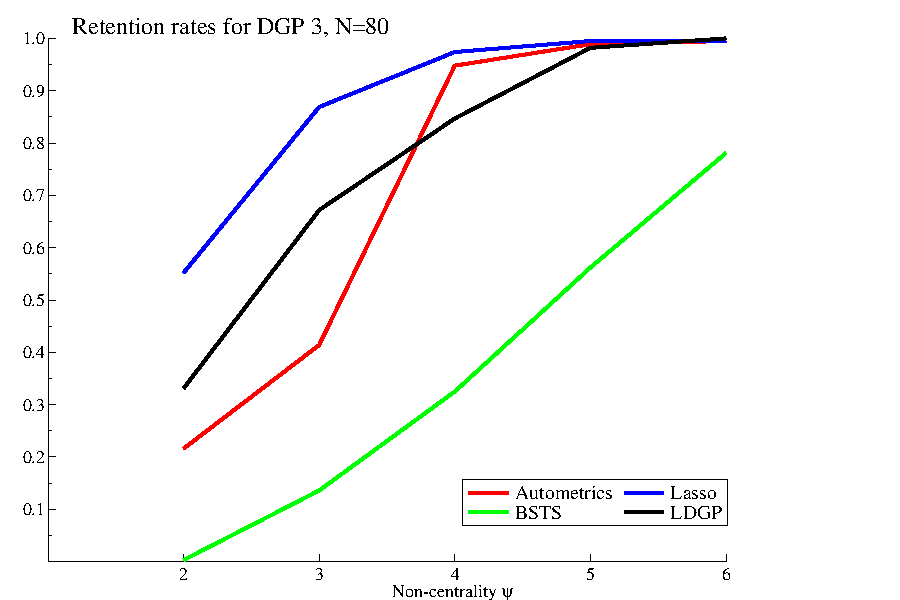
\includegraphics[scale=0.5]{RetRatesDGP3a}
\caption{Retention rates for DGP 3}
\label{fig:RetRatesDGP3a}

\end{minipage}

\end{figure}

\clearpage

The above results show the Lasso consistently achieves the highest potency and has the highest retention rates across all levels of $\psi$ but also has by far the highest gauge. Autometrics selects relevant regressors at a level which is generally similar to the theoretical retention probability (with a couple of exceptions) and does nearly as well as the Lasso when $\psi>4$. In comparison to Lasso and Autometrics, BSTS does not fare well when selecting relevant variables, even for variables with high values of $\psi$. Retention rates and potency measures do not change drastically between $N<T$ and $N>T$ when $\psi>4$, but results for lower values of $\psi$ vary quite significantly. 

BSTS consistently achieves the lowest gauge but its low potency and retention rates indicate that it tends to select very sparse models in general. Note that when conducting the experiments, various priors were tested but this did not seem to have an impact on the results for BSTS. The gauge for Lasso is generally very high and in the range of $0.12$ to $0.22$, which along with the high levels of potency indicate that it selects models which include a lot of variables. In all of the six experiments, Autometrics has a gauge close to the significance level $\alpha = 0.01$, however in DGP 2 with $\psi = 2$, the gauge is slightly higher at $0.029$ probably because it misses some relevant variables with such low non-centralities. It could also possibly correspond to a `bad draw' due to the fact that fixed regressors are used. 

The RCMSE results are most easily interpreted by the graphs, which show that the results vary depending on values of $\psi$. As can be seen in Figures \ref{RCMSECase1a} and \ref{fig:CMSEDGP3a}, Autometrics performs well for high values of $\psi$. Figure \ref{fig:CMSEDGP3a} shows that Lasso and BSTS increasingly struggle as $\psi$ rises. Results are mixed in Figure \ref{fig:RCMSECase2a}, where there is a low non-centrality of $\psi=2$. Note that the spike in RCMSE for $x_{2}$ in Autometrics could be due to the fact that fixed regressors are used. 

Both the Lasso and Autometrics have results similar to, or better than, the benchmark when examining the potency and retention rates. As mentioned, across the board, the Lasso has high potencies and high gauges, meaning that overall there is less `selection' going on. It is a different story when examining the RCMSE results however; Autometrics is much closer to the benchmark (except in the case where $\psi=2$ where results are varied). This means the costs of inference are high in Lasso and BSTS.

The five biggest takeaways from this set of experiments are:
\begin{enumerate}
\item Autometrics consistently has a gauge close to the significance level and retention rates/potencies close to the theoretical retention probabilities.
\item The Lasso scores high for successfully retaining relevant variables, but taken next to the gauges, this is less impressive.
\item BSTS selects models which are very sparse, which is seen clearly through its extremely low measures for gauge, and relatively low levels of potency.
\item The costs of inference vary with $\psi$, but generally are quite low with Autometrics, but high for both the Lasso and BSTS.
\item The huge differences in gauge between the Lasso and BSTS make comparisons using just these two measures impossible. It is infeasible to derive a `gauge-corrected' potency that would make comparisons meaningful.
\end{enumerate}



\subsection{Correlation Between Relevant Regressors}

The second set of experiments considers several cases where there is correlation between the relevant regressors. There are two different DGPs considered, which again vary according to their coefficients $\beta_{1},...,\beta_{5}$ and therefore their respective non-centralities. In both DGPs $\beta_{0}=1$ and $\delta = 0.5$. $\beta_{1},...,\beta_{5}$ have been chosen so that the non-centralities in this set of experiments are in line with those in the first set of experiments, making the results comparable. In all experiments fixed regressors are used. As in the first set of experiments, the two DGPs are nested in two different GUMs with $N=80$ and $N=120$. In all experiments, $T=100$. Thus, there are four separate experiments performed and reported on.   Let $\textbf{x}_{t}'=(x_{1,t},...,x_{N,t})$. The DGPs take the following form: 
$$y_{t}=\beta_{0} + \delta y_{t-1}+\beta_{1}x_{1,t}+\beta_{2}x_{2,t}+ \beta_{3}x_{3,t}+ \beta_{4}x_{4,t}+ \beta_{5}x_{5,t} + \epsilon_{t}$$
$$\epsilon_{t} \sim \mathsf{IN}[0,1] $$
 $$\textbf{x}_{t} \sim \mathsf{IN}_{N} [0,\Omega]$$
with $\omega_{kk} = 1 $, $\omega_{jk} = 0.9 $ for $j \neq k$, $j,k \leq 5$ and $\omega_{jk} = 0 $ elsewhere. Due to the correlation between regressors, it is difficult to derive a formula which analytically gives the relationship between $\psi_{k}$, $\sigma_{\widehat{\beta}_{k}}$, and $t_{\beta_{k}}$. However, $\psi_{k}$ can also be expressed as $\mathsf{E}$[$t_{\widehat{\beta}_{k}}$]. Thus the $\beta_{k}$s in this set of experiment are set such that the average $t$-statistic for variable $x_{k}$ across simulations is equal to the desired $\psi$. More explicitly:
$$\psi_{k} = \mathsf{E}[t_{\widehat{\beta}_{k}}] = \frac{1}{1000}\sum_{i=1}^{1000}t_{\widehat{\beta}_{k},i}$$
where $t_{\widehat{\beta}_{k},i}$ is the calculated $t$-statistic for $\widehat{\beta}_{k}$ in simulation $i$. Table \ref{DGPs4and5} describes the two DGPs considered.
%TABLE DGPs of experiments including orthogonal variables
\begin{table}[h]
\centering
\begin{tabular}{c|c|c|c|c|c|c}

&  &$x_{1}$ &$x_{2}$ &$x_{3}$ &  $x_{4}$ & $x_{5}$  \\
\hline
\textbf{DGP 4} & $\beta_{k}$  & 0.58 &0.84 &1.25 &  1.55 & 1.75 \\

 	& $\psi_{k}$ &2 &3 &4 &5 &6 \\
\hline
\textbf{DGP 5} & $\beta_{k}$  & -0.58 &0.84 &-1.25 &  1.55 &-1.75 \\

 	& $\psi_{k}$  &-2 &3 &-4 &5 &-6 \\

    
\end{tabular}
\caption{DGP specification for experiments with correlation between relevant regressors}
\label{DGPs4and5}
\end{table} 

When the regressors are not orthogonal, as explained, simply using 1-cut selection on the DGP is not a feasible baseline. The `best case scenario' then is doing selection on the DGP using the algorithms themselves. These results capture how effective the algorithm is in the case where the GUM includes exactly the correct regressors. The difference between the RCMSE from selection on the DGP and selection from the GUM is therefore a measure of the costs of inference. 

%For CMSE - no selection on LDGP is benchmark. 




Tables \ref{DGP4GP} and \ref{tDGP4RR} report the gauge, potency and retention rates for DGP 4, and include results when selecting from the DGP for each algorithm. Tables \ref{DGP5GP} and \ref{DGP5RetRates} do the same for DGP 5. Tables \ref{DGP4CMSE} and \ref{LDGP5CMSE} report RCMSE results. The lowest gauge, highest potency, and lowest RCMSE are in bold. Figures \ref{fig:RetRatesDGP4a}-\ref{fig:CMSEDGP5a} graph the results. Figures \ref{fig:CMSEDiffDGP4a} and \ref{fig:CMSEDiffDGP5a} graph the differences between RCMSE for each algorithm and their base line, and thus give an indication of the costs of inference for each of the algorithms.
% Table generated by Excel2LaTeX from sheet 'GPDGP4'
\begin{table}[h]
  \centering
\begin{tabular}{r|r|r|r|r}

         & \multicolumn{2}{|c|}{\textbf{$N=80$}} & \multicolumn{2}{|c}{\textbf{$N=120$}} \\
            & Potency           & Gauge           & Potency            & Gauge           \\
          \hline
    \textbf{Autometrics} & 0.777 & 0.014 & 0.769 & 0.013 \\
    \textit{from DGP} & 0.797 &       & 0.797 &  \\
    \hline
    \textbf{Lasso} & \textbf{0.993} & 0.108 & \textbf{0.993} & 0.077 \\
    \textit{from DGP} & 0.994 &       & 0.994 &  \\
    \hline
    \textbf{BSTS} & 0.690 & \textbf{0.000} & 0.677 & \textbf{0.000} \\
    \textit{from DGP} & 0.784 &       & 0.784 &  \\

    \end{tabular}%
      \caption{Gauge and potency for DGP 4}
  \label{DGP4GP}%
  
\end{table}%
% Table generated by Excel2LaTeX from sheet 'RetRatesChartDGP4'
\begin{table}[h]
  \centering

    \begin{tabular}{r|r|rrrrr}

          & \boldmath{}\textbf{$\psi$}\unboldmath{} & 2     & 3     & 4     & 5     & 6 \\
          \hline

          & $\textsf{P}_{0.01}$ & 0.266 & 0.645 & 0.914 & 0.990 & 0.999  \\
          \hline
    $\bm{N=80} $& \textbf{Autometrics} & 0.333 & 0.568 & 0.988 & 0.998 & 0.998 \\
    \textbf{} & \textbf{Lasso} & \textbf{0.977} & \textbf{0.990} & \textbf{1.000} & \textbf{1.000} & \textbf{1.000} \\
    \textbf{} & \textbf{BSTS} & 0.179 & 0.340 & 0.949 & 0.993 & 0.991 \\
    \hline
   $ \bm{N=120}$ & \textbf{Autometrics} & 0.316 & 0.611 & 0.923 & 0.996 & 0.999 \\
    \textbf{} & \textbf{Lasso} & \textbf{0.968} & \textbf{0.998} & \textbf{1.000} & \textbf{1.000} & \textbf{1.000} \\
    \textbf{} & \textbf{BSTS} & 0.155 & 0.369 & 0.874 & 0.988 & 0.999 \\
    \hline
    \textbf{From DGP} & \textbf{Autometrics} & 0.330 & 0.723 & 0.934 & 0.996 & 1.000 \\
          & \textbf{Lasso} & 0.979 & 0.993 & 1.000 & 1.000 & 1.000 \\
          & \textbf{BSTS} & 0.344 & 0.589 & 0.990 & 0.999 & 0.998 \\

    \end{tabular}%
      \caption{Retention rates for DGP 4, including from DGP}
  \label{tDGP4RR}%
\end{table}%


% Table generated by Excel2LaTeX from sheet 'GPDGP5'
\begin{table}[htbp]
  \centering

    \begin{tabular}{r|r|r|r|r}

         & \multicolumn{2}{|c|}{\textbf{$N=80$}} & \multicolumn{2}{|c}{\textbf{$N=120$}} \\
            & Potency           & Gauge           & Potency            & Gauge           \\
          \hline
    \textbf{Autometrics} & \textbf{0.716} & 0.014 & \textbf{0.719} & 0.014 \\
    \textit{from DGP} & 0.775 &       & 0.775 &  \\
    \hline
    \textbf{Lasso} & 0.429 & 0.088 & 0.374 & 0.057 \\
    \textit{from DGP} & 0.986 &       & 0.986 &  \\
    \hline
    \textbf{BSTS} & 0.531 & \textbf{0.000}   & 0.439 &\textbf{0.000} \\
    \textit{from DGP} & 0.675 &       & 0.675 &  \\

    \end{tabular}%
      \caption{Gauge and potency for DGP 5}
  \label{DGP5GP}%
\end{table}%






% Table generated by Excel2LaTeX from sheet 'RetRatesDGP5Chart'
\begin{table}[htbp]
  \centering

    \begin{tabular}{r|r|rrrrr}

          & \boldmath{}\textbf{$\psi$}\unboldmath{} & -2    & 3     & -4    & 5     & -6 \\
          \hline

        & $\mathsf{P}_{0.01}$ & 0.266 & 0.645 & 0.914 & 0.990 & 0.999  \\
        \hline
    $\bm{N=80} $& \textbf{Autometrics} & \textbf{0.255} & \textbf{0.355} & 0.981 & \textbf{0.996} & 0.994 \\
    \textbf{} & \textbf{Lasso} & 0.065 & 0.013 & \textbf{0.984} & 0.095 & \textbf{0.988} \\
    \textbf{} & \textbf{BSTS} & 0.022 & 0.056 & 0.798 & 0.827 & 0.951 \\
    \hline
    $\bm{N=120}$ & \textbf{Autometrics} & \textbf{0.290} & \textbf{0.482} & \textbf{0.841} & \textbf{0.984} & \textbf{1.000} \\
    \textbf{} & \textbf{Lasso} & 0.254 & 0.007 & 0.590 & 0.019 & 0.998 \\
    \textbf{} & \textbf{BSTS} & 0.054 & 0.061 & 0.353 & 0.727 & 0.999 \\
    \hline
    \textbf{From DGP} & \textbf{Autometrics} & 0.336 & 0.631 & 0.925 & 0.981 & 1.000 \\
          & \textbf{Lasso} & 0.967 & 0.963 & 1.000 & 1.000 & 1.000 \\
          & \textbf{BSTS} & 0.150 & 0.267 & 0.974 & 0.989 & 0.995 \\
 
    \end{tabular}%
      \caption{Retention Rates for DGP 5, including from DGP}
  \label{DGP5RetRates}%
\end{table}%



% Table generated by Excel2LaTeX from sheet 'CMSEChartDGP4'
\begin{table}[htbp]
  \centering

   \begin{tabular}{r|r|rrrrrr}

          &       & $y_{t-1}$ & $x_{1}$ & $x_{2}$ & $x_{3}$ & $x_{4}$ & $x_{5}$ \\
          & $\delta/\beta_{k}$ &   0.5 & 0.58 &0.84 &1.25 &  1.55 & 1.75  \\
           \hline
    $\bm{N=80} $& \textbf{Autometrics} & \textbf{0.017} & 0.438 & 0.423 & 0.277 & 0.377 & 0.377 \\
    \textbf{} & \textbf{Lasso} & 0.038 & \textbf{0.279} & \textbf{0.339} & \textbf{0.259} & \textbf{0.292} & \textbf{0.307} \\
    \textbf{} & \textbf{BSTS} & 0.024 & 0.441 & 0.572 & 0.448 & 0.624 & 0.541 \\
    \hline
    $\bm{N=120}$ & \textbf{Autometrics} & \textbf{0.016} & 0.432 & 0.332 & 0.431 & 0.405 & \textbf{0.342} \\
    \textbf{} & \textbf{Lasso} & 0.038 & \textbf{0.272} & \textbf{0.314} & \textbf{0.333} &\textbf{ 0.313} & 0.354 \\
    \textbf{} & \textbf{BSTS} & 0.020 & 0.530 & 0.555 & 0.606 & 0.626 & 0.499 \\
    \hline
    \textbf{From DGP} & \textbf{Autometrics} & 0.016 & 0.442 & 0.317 & 0.366 & 0.364 & 0.326 \\
          & \textbf{Lasso} & 0.021 & 0.266 & 0.329 & 0.255 & 0.286 & 0.297 \\
          & \textbf{BSTS} & 0.026 & 0.395 & 0.504 & 0.375 & 0.484 & 0.432 \\

    \end{tabular}%
      \caption{RCMSE for DGP 4, including baseline}
  \label{DGP4CMSE}%
\end{table}%


% Table generated by Excel2LaTeX from sheet 'CMSEDGP5Chart'
\begin{table}[htbp]
  \centering

    \begin{tabular}{r|r|rrrrrrr}

          &       & $y_{t-1}$ & $x_{1}$ & $x_{2}$ & $x_{3}$ & $x_{4}$ & $x_{5}$ &  \\

         & $\delta/\beta_{k}$ &   0.5 & -0.58 &0.84 &-1.25 &  1.55 & -1.75  \\
         \hline
    $\bm{N=80} $& \textbf{Autometrics} & 0.334 & \textbf{0.281} & \textbf{0.316} & \textbf{0.287} & \textbf{0.325} & \textbf{0.258} &  \\
    \textbf{} & \textbf{Lasso} & 0.120 & 0.463 & 0.656 & 0.778 & 1.074 & 1.225 &  \\
    \textbf{} & \textbf{BSTS} & \textbf{0.078} & 0.288 & 0.527 & 0.446 & 0.572 & 0.571 &  \\
    \hline
    $\bm{N=120}$ & \textbf{Autometrics} & 0.273 & \textbf{0.292} & \textbf{0.303} & \textbf{0.296} & \textbf{0.341} & \textbf{0.257} &  \\
    \textbf{} & \textbf{Lasso} & 0.226 & 0.424 & 0.554 & 1.030 & 1.029 & 0.955 &  \\
    \textbf{} & \textbf{BSTS} & \textbf{0.097} & 0.405 & 0.510 & 0.603 & 0.722 & 0.496 &  \\
    \hline
    \textbf{From DGP} & \textbf{Autometrics} & 0.051 & 0.342 & 0.239 & 0.330 & 0.334 & 0.330 &  \\
          & \textbf{Lasso} & 0.052 & 0.286 & 0.362 & 0.266 & 0.307 & 0.326 &  \\
          & \textbf{BSTS} & 0.071 & 0.342 & 0.482 & 0.384 & 0.411 & 0.408 &  \\

    \end{tabular}%
      \caption{RCMSE for DGP 5, including from DGP}
  \label{LDGP5CMSE}%
\end{table}%






\begin{figure}

\begin{minipage}{.5\textwidth}
\centering
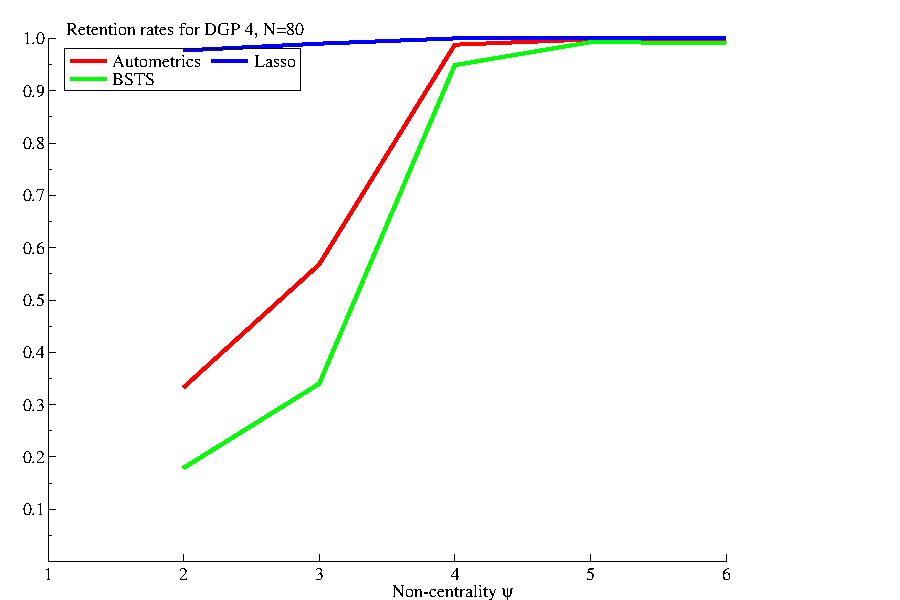
\includegraphics[scale=0.5]{RetRatesDGP4a}
\caption{Retention rates DGP 4 \newline $N=80$}
\label{fig:RetRatesDGP4a}
\end{minipage}%
\begin{minipage}{.5\textwidth}
\centering
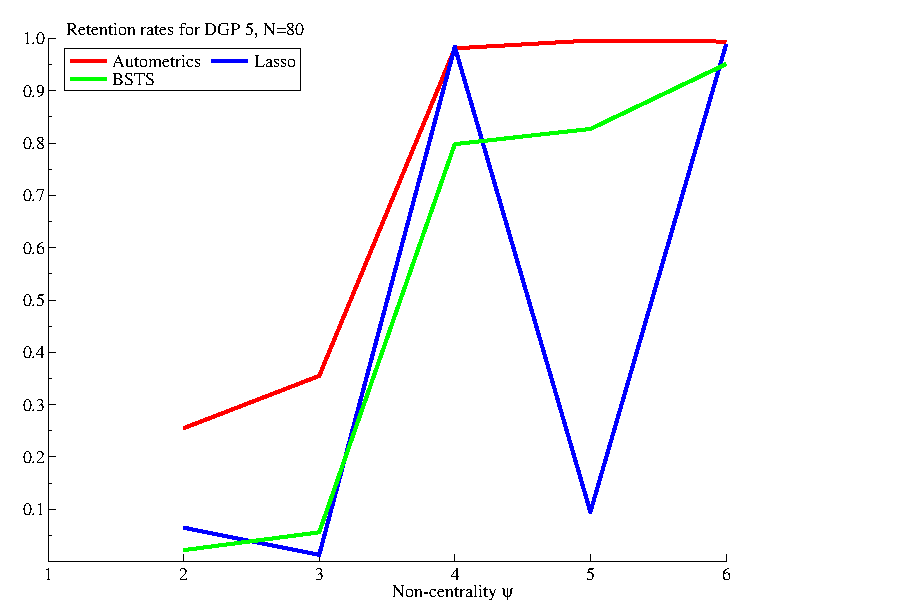
\includegraphics[scale=0.5]{RetRatesDGP5a}
\caption{Retention Rates DGP 5 \newline $N=80$}
\label{fig:RetRatesDGP5a}

\end{minipage}

\end{figure}

\begin{figure}

\begin{minipage}{.5\textwidth}
\centering
\includegraphics[scale=0.5]{RCMSEDGP4a}
\caption{RCMSE for DGP 4 \newline $N=80$}
\label{fig:CMSEDGP4a}
\end{minipage}%
\begin{minipage}{.5\textwidth}
\centering
\includegraphics[scale=0.5]{RCMSEDGP5a}
\caption{RCMSE for DGP 5 \newline $N=80$}
\label{fig:CMSEDGP5a}

\end{minipage}

\end{figure}

\begin{figure}

\begin{minipage}{.5\textwidth}
\centering
\includegraphics[scale=0.5]{RCMSEDiffDGP4a}
\captionsetup{justification=centering}
\caption{RCMSE Differences for DGP 4 \newline $N=80$}
\label{fig:CMSEDiffDGP4a}
\end{minipage}%
\begin{minipage}{.5\textwidth}
\centering
\includegraphics[scale=0.5]{RCMSEDiffDGP5a}
\captionsetup{justification=centering}
\caption{RCMSE Differences for DGP 5 \newline $N=80$}
\label{fig:CMSEDiffDGP5a}

\end{minipage}

\end{figure}

\clearpage
%Note that this section only examines results within the set of experiments where there is correlation between relevant regressors; analysis and comparison across the three sets of experiments will be discussed later on. 

When considering DGP 4 results, when $\psi_{k} > 0, \forall k$, the Lasso has both the highest measures of potency and gauge. BSTS has the lowest gauge and Autometric's gauge is close to the significance level $\alpha$. Going from $N<T$ to $N>T$ in most cases does not have a big impact on the results. Both Autometrics and the Lasso have retention rates similar to their benchmark, while the benchmark for BSTS gives quite different results. The graph for the RCMSE differences is interesting, and shows there are almost no costs of search for the Lasso, and for Autometrics there are in fact negative costs of search, meaning that sometimes parameter estimates are even more accurate than in the theoretical best case scenario. This is likely due to adventitiously selecting irrelevant variables which partly proxy a relevant variable which has not been selected, which results in a smaller error variance.

When looking at DGP 5, it is clear that the algorithms struggle to varying degrees with alternating signs. This is particularly true for the Lasso, with retention rates on regressors with $\psi>0$ being very low, irrespective of their magnitude, when the largest $\psi$ in the experiment is negative. The search costs of the Lasso also increase with $|\psi|$. The results for the gauge are similar to previous experiments; the gauge for BSTS is low in every experiment, the gauge for Autometrics is slightly higher than the significance level $\alpha$, and the gauge for the Lasso varies across the experiments. The costs of search for both Autometrics and BSTS, as measured by the RCMSE differences, are quite low. 

Comparing the results from DGP 4 to DGP 5 is striking. While intuitively and theoretically the DGPs have nearly identical properties, the actual results vary drastically. Thinking about non-centrality as the signal-to-noise ratio, whether a variable has a positive or negative non-centrality should not have an impact on how often it is selected by an algorithm; it is the magnitude of the the signal-to-noise ratio, $|\psi|$, which should influence an algorithm's ability to select that variable. Indeed, in the case of orthogonal variables alternating signs did not result in potency and retention rate measures which were notably different from cases where the signs were all the same. 

It is immediately clear however that something peculiar is going on with DGP 5 when the signs are alternating. DGP 4 has retention rates as expected are increasing with $\psi$. In DGP 5 while both Autometrics and BSTS have higher retention rates as $|\psi|$ rises, the Lasso struggles to select either of the regressors with $\psi>0$. It should also be noted that while the retention rates do increase with $|\psi|$ for Autometrics and BSTS, the increase is not at all `uniform' and both Autometrics and BSTS are more successful at selecting variables with $\psi<0$. The RCMSE results illustrate the parameter estimates also vary across the DGPs. In DGP 4, the Lasso has the lowest RCMSE for all variables, while it has the highest RCMSEs for all variables in DGP 5. Furthermore, the RCMSEs increase with $\psi$ for the Lasso with alternating signs. 

The reason why the Lasso has such difficulty selecting the regressors with negative signs is due to the nature of the search its algorithm uses to identify non-zero coefficients. The algorithm identifies the regressor which is `most significant' and shrinks the coefficients of regressors which are highly correlated with the identified regressor to zero. Certain implementations of the Lasso have built in features to account for this when the coefficients of the correlated regressors have the same sign (i.e. see Hastie and Zou (2005)) but no algorithm exists to account for regressors which have coefficients with opposite signs. In the case of DGP 5, the Lasso (correctly) identifies $x_{5}$ with $\psi_{5} = -6$ as the most significant, and since $x_{5}$ is highly correlated with $x_{1},...,x_{4}$, it shrinks their coefficients to zero. Because the Lasso allows for variables which are significant `in the same direction' (i.e. in this case negatively significant), to be effectively `re-added', variables $x_{1}$ and $x_{3}$ which have respective non-centralities of -2 and -4 are selected, but there is no mechanism for $x_{2}$ and $x_{4}$ with their positive coefficients to be `reconsidered' for selection. If it was the case that the most significant variable had a positive coefficient, then any variables with negative coefficients would be shrunk to zero and not selected. That is, negative coefficients and positive correlations are isomorphic to positive coefficients and negative correlations, so this result would also hold if it parameter signs were switched.

The biggest takeaways from this second set of experiments are:
\begin{enumerate}
\item Selection when signs alternate produces remarkably different results, especially for the Lasso. 
%This is likely due to the nature by which Lasso's algorithm works; omitting one of a pair of 
\item When $\psi_{k} > 0 \ \forall \ k$ the Lasso selects a lot of both relevant and irrelevant variables, BSTS does not select many of either, and Autometrics is somewhere in the middle. 
\item In terms of their RCMSEs, the behaviour of Autometrics commencing from the GUM is relatively similar to starting from the DGP. The retention rates for relevant variables in both these cases are close to the theory-derived retention probabilities.
\item Remarkably, across all experiments, there is little difference in the performance of Autometrics between $N<T$ and $N>T$ ($N=80$ and $N=120$). 
\item As found in the previous set of experiments, search costs for Autometrics can sometimes be negative.
\item The RCMSEs for Autometrics are relatively constant across all $\psi$ and for the Lasso and BSTS they are not. 
\end{enumerate}



\subsection{Correlation Between all Regressors}


The third set of experiments considers several cases where there is correlation between all regressors. There are two different DGPs considered, which again vary according to the coefficients $\beta_{1},...,\beta_{5}$ and therefore their respective non-centralities. Fixed regressors are used in all experiments. These two DGPs are nested, as previously, in two different GUMs with $N=80$ and $N=120$. In all experiments, $T=100$. There are four separate experiments performed and reported on. Let $\textbf{x}_{t}'=(x_{1,t},...,x_{N,t})$. The DGPs take the following form: 
$$y_{t}=\beta_{0} + \delta y_{t-1}+\beta_{1}x_{1,t}+\beta_{2}x_{2,t}+ \beta_{3}x_{3,t}+ \beta_{4}x_{4,t}+ \beta_{5}x_{5,t} + \epsilon_{t}$$
$$\epsilon_{t} \sim \mathsf{IN}[0,1] $$
 $$\textbf{x}_{t} \sim \mathsf{IN}_{N}[0,\Omega]$$
with $\omega_{kk} = 1 $, $\omega_{jk} = 0.8 $ for $k \neq j $. The biggest difference between this set of experiments and previous set is that here $\Omega$ is a full $N \times N$ matrix. As with the second set of experiments,  determining the relationship between $\psi_{k}$, $\beta_{k}$ and $\sigma_{\hat{\beta_{k}}}$ is difficult to do analytically because of the correlation structure. Thus $\beta_{1},...,\beta_{5}$ in this set of experiment are set such that the average $t$-statistic for variable $x_{k}$ across simulations aligns with the non-centralities in the previous experiments. More explicitly:
$$\psi_{k} = \mathsf{E}[t_{\widehat{\beta}_{k}}] = \frac{1}{1000}\sum_{i=1}^{1000}t_{\widehat{\beta}_{k},i}$$
where $t_{\widehat{\beta}_{k},i}$ is the calculated $t$-statistic for $\widehat{\beta}_{k}$ in simulation $i$. Table \ref{DGP67} describes the two DGPs considered, with the $\beta_{k}$s that correspond to the desired $\psi_{k}$s. 



The following table describes the two DGPs considered, from hereon referred to as DGP 6 and 7:


%TABLE DGPs of experiments including orthogonal variables
\begin{table}[h]



\centering
\begin{tabular}{c|c|c|c|c|c|c}

&  &$x_{1}$ &$x_{2}$ &$x_{3}$ &  $x_{4}$ & $x_{5}$  \\
\hline
\textbf{DGP 6} & $\beta_{k}$  & 0.4&0.6 &0.9&1.1  &1.25  \\

 	& $\psi_{k}$  &2 &3 &4 &5 &6 \\
\hline
\textbf{DGP 7} & $\beta_{k}$  & -0.4&0.6 &-0.9&1.1  &-1.25 \\

 	& $\psi_{k}$ &-2 &3 &-4 &5 &-6 \\

    
\end{tabular}
\caption{DGP specification for experiments with correlation between all regressors}
\label{DGP67}
\end{table} 
The following tables report the potency, gauge, retention rates and RCMSE for DGP 6 and DGP 7. The lowest gauge, highest potency and lowest RCMSE are in bold. Again in this set of experiments the significance level for Autometrics was set to $\alpha= 0.01$. The results are also graphed. 
\\
% Table generated by Excel2LaTeX from sheet 'DGP6GP'
\begin{table}[htbp]
  \centering

    \begin{tabular}{r|r|r|r|r}

         & \multicolumn{2}{|c|}{$N=80$} & \multicolumn{2}{|c}{$N=120$}  \\
            & Potency           & Gauge           & Potency            & Gauge           \\
          \hline
    \textbf{Autometrics} & 0.736 & 0.016 & 0.718 & 0.015 \\
    \textit{from DGP} & 0.798 &       & 0.798 &  \\
    \hline
    \textbf{Lasso} & \textbf{0.909} & 0.182 & \textbf{0.894} & 0.131 \\
    \textit{from DGP} & 0.993 &       & 0.993 &  \\
    \hline
    \textbf{BSTS} & 0.653 & \textbf{0.004} & 0.631 & \textbf{0.005} \\
    \textit{from DGP} & 0.764 &       & 0.764 &  \\

    \end{tabular}%
      \caption{Gauge and potency for DGP 6}
  \label{DGP6GP}%
\end{table}%




% Table generated by Excel2LaTeX from sheet 'RetRatesDGP6Chart'
\begin{table}[htbp]
  \centering

    \begin{tabular}{r|r|rrrrr}

          & \boldmath{}\textbf{$\psi$}\unboldmath{} & 2    & 3     & 4    & 5     & 6 \\
          \hline

          & $\mathsf{P}_{0.01}$ & 0.266 & 0.645 & 0.914 & 0.990 & 0.999  \\
          \hline
    $\bm{N=80}$ & \textbf{Autometrics} & 0.262 & 0.439 & 0.985 & 0.996 & 0.996 \\
    \textbf{} & \textbf{Lasso} & \textbf{0.766} & \textbf{0.778} & \textbf{1.000} & \textbf{1.000} & \textbf{1.000} \\
    \textbf{} & \textbf{BSTS} & 0.116 & 0.251 & 0.923 & 0.984 & 0.990 \\
    \hline
    $\bm{N=120}$ & \textbf{Autometrics} & 0.212 & 0.524 & 0.890 & 0.966 & 0.999 \\
    \textbf{} & \textbf{Lasso} & \textbf{0.560} & \textbf{0.924} & \textbf{0.991} & \textbf{0.998} & \textbf{0.999} \\
    \textbf{} & \textbf{BSTS} & 0.093 & 0.285 & 0.810 & 0.971 & 0.997 \\
    \hline
    \textbf{From DGP} & \textbf{Autometrics} & 0.327 & 0.729 & 0.938 & 0.995 & 1.000 \\
          & \textbf{Lasso} & 0.969 & 0.994 & 1.000 & 1.000 & 1.000 \\
          & \textbf{BSTS} & 0.281 & 0.554 & 0.990 & 0.998 & 0.999 \\

    \end{tabular}%
      \caption{Retention Rates for DGP 6}
  \label{DGP6RetRates}%
\end{table}%

% Table generated by Excel2LaTeX from sheet 'CMSEDGP6Chart'
\begin{table}[htbp]
  \centering

    \begin{tabular}{r|r|rrrrrr}
  
          &       & $y_{t-1}$ & $x_{1}$ & $x_{2}$ & $x_{3}$ & $x_{4}$ & $x_{5}$ \\

          &   $\delta/\beta_{k} $   & 0.5 & 0.4&0.6 &0.9&1.1  &1.25  \\
          \hline
    $\bm{N=80}$ & \textbf{Autometrics} & \textbf{0.025} & 0.318 & \textbf{0.313} & \textbf{0.190} & \textbf{0.241} & \textbf{0.250} \\
    \textbf{} & \textbf{Lasso} & 0.041 & \textbf{0.230} & 0.347 & 0.257 & 0.349 & 0.315 \\
    \textbf{} & \textbf{BSTS} & 0.036 & 0.318 & 0.404 & 0.386 & 0.386 & 0.348 \\
    \hline
    $\bm{N=120}$ & \textbf{Autometrics} & \textbf{0.023} & 0.329 & \textbf{0.227} & \textbf{0.263} & \textbf{0.254} & \textbf{0.232} \\
    \textbf{} & \textbf{Lasso} & 0.033 & \textbf{0.254 }& 0.313 & 0.376 & 0.462 & 0.389 \\
    \textbf{} & \textbf{BSTS} & 0.026 & 0.306 & 0.370 & 0.430 & 0.428 & 0.346 \\
    \hline
    \textbf{From DGP} & \textbf{Autometrics} & 0.024 & 0.307 & 0.219 & 0.259 & 0.255 & 0.230 \\
          & \textbf{Lasso} & 0.029 & 0.192 & 0.234 & 0.182 & 0.204 & 0.211\\
          & \textbf{BSTS} & 0.036 & 0.275 & 0.361 & 0.258 & 0.337 & 0.314 \\
 
    \end{tabular}%
      \caption{RCMSE for DGP 6}
  \label{DGP6CMSE}%
\end{table}%


% Table generated by Excel2LaTeX from sheet 'GPDGP7'
\begin{table}[htbp]
  \centering
 
    \begin{tabular}{r|r|r|r|r}

         & \multicolumn{2}{|c|}{$N=80$} & \multicolumn{2}{|c}{$N=120$}  \\
            & Potency           & Gauge           & Potency            & Gauge           \\
          \hline
    \textbf{Autometrics} & 0.718 & 0.014 & 0.707 & 0.014 \\
    \textit{from DGP} & 0.778 &    & 0.778 &  \\
    \hline
    \textbf{Lasso} & \textbf{0.787} & 0.154 & \textbf{0.823} & 0.131 \\
    \textit{from DGP} & 0.986 &    & 0.986 &  \\
    \hline
    \textbf{BSTS} & 0.512 & \textbf{0.001} & 0.401 & \textbf{0.001} \\
    \textit{from DGP} & 0.657 &   & -0.657 &  \\

    \end{tabular}%
     \caption{Gauge and potency for DGP 7}
  \label{DGP7GP}%
\end{table}%


% Table generated by Excel2LaTeX from sheet 'RetRatesDGP7Chart'
\begin{table}[htbp]
  \centering

    \begin{tabular}{r|r|rrrrr}

          & \boldmath{}\textbf{$\psi$}\unboldmath{} & -2    & 3     & -4    & 5     & -6 \\
          \hline

          & $\mathsf{P}_{0.01}$ & 0.266 & 0.645 & 0.914 & 0.990 & 0.999  \\
          \hline
    \textbf{N=80} & \textbf{Autometrics} & 0.230 & 0.380 & 0.988 & 0.993 & 0.998 \\
    \textbf{} & \textbf{Lasso} & \textbf{0.507} & \textbf{0.466} & \textbf{0.999} & \textbf{0.963} & \textbf{1.000} \\
    \textbf{} & \textbf{BSTS} & 0.011 & 0.041 & 0.812 & 0.791 & 0.907 \\
    \hline
    \textbf{N=120} & \textbf{Autometrics} & 0.253 & 0.510 & 0.803 & 0.972 & 0.999 \\
    \textbf{} & \textbf{Lasso} & \textbf{0.603} & \textbf{0.683} & \textbf{0.904} & \textbf{0.926} & \textbf{1.000} \\
    \textbf{} & \textbf{BSTS} & 0.037 & 0.051 & 0.303 & 0.641 & 0.971 \\
    \hline
    \textbf{From DGP} & \textbf{Autometrics} & 0.330 & 0.649 & 0.931 & 0.980 & 1.000 \\
          & \textbf{Lasso} & 0.964 & 0.967 & 1.000 & 1.000 & 1.000 \\
          & \textbf{BSTS} & 0.103 & 0.242 & 0.965 & 0.983 & 0.993 \\

    \end{tabular}%
     \caption{Retention Rates for DGP 7}
  \label{DGP7RetRates}%
\end{table}%

% Table generated by Excel2LaTeX from sheet 'CMSEDGP7Chart'
\begin{table}[htbp]
  \centering

    \begin{tabular}{r|r|rrrrrr}

          &       & $y_{t-1}$ & $x_{1}$ & $x_{2}$ & $x_{3}$ & $x_{4}$ & $x_{5}$ \\

     &     & 0.5 & -0.4&0.6 &-0.9&1.1  &-1.25  \\
     \hline
    $\bm{N=80}$ & \textbf{Autometrics} & \textbf{0.059} & 0.286 & \textbf{0.267} & \textbf{0.187} & \textbf{0.224} & \textbf{0.246} \\
    \textbf{} & \textbf{Lasso} & 0.078 & 0.257 & 0.415 & 0.330 & 0.514 & 0.532 \\
    \textbf{} & \textbf{BSTS} & 0.111 & \textbf{0.188} & 0.358 & 0.327 & 0.405 & 0.438 \\
    \hline
     $\bm{N=120}$ & \textbf{Autometrics} & \textbf{0.070} & 0.328 & \textbf{0.230} & \textbf{0.221} & \textbf{0.253} &\textbf{ 0.232} \\
    \textbf{} & \textbf{Lasso} & 0.121 & \textbf{0.257} & 0.370 & 0.526 & 0.564 & 0.421 \\
    \textbf{} & \textbf{BSTS} & 0.147 & 0.272 & 0.362 & 0.458 & 0.515 & 0.359 \\
    \hline
    \textbf{From DGP} & \textbf{Autometrics} & 0.059 & 0.246 & 0.168 & 0.237 & 0.236 & 0.232 \\
          & \textbf{Lasso} & 0.059 & 0.205 & 0.256 & 0.190 & 0.216 & 0.229 \\
          & \textbf{BSTS} & 0.084 & 0.236 & 0.344 & 0.281 & 0.294 & 0.298 \\

    \end{tabular}%
      \caption{RCMSE for DGP 7}
  \label{DGP7CMSE}%
\end{table}%













\begin{figure}[h]

\begin{minipage}{.5\textwidth}
\centering
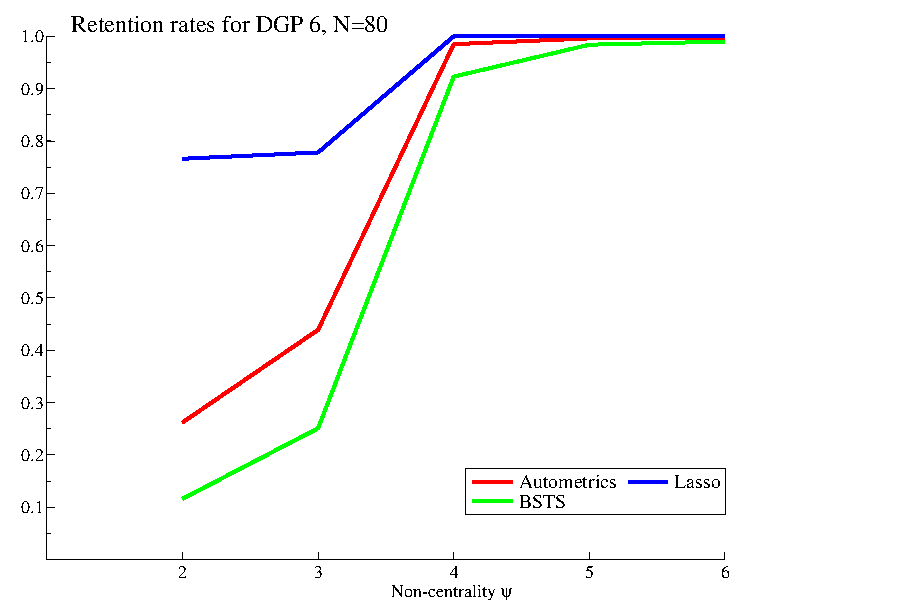
\includegraphics[scale=0.5]{RetRatesDGP6a}
\caption{Retention rates DGP 6 \newline $N=80$}
\label{fig:RetRatesDGP6a}
\end{minipage}%
\begin{minipage}{.5\textwidth}
\centering
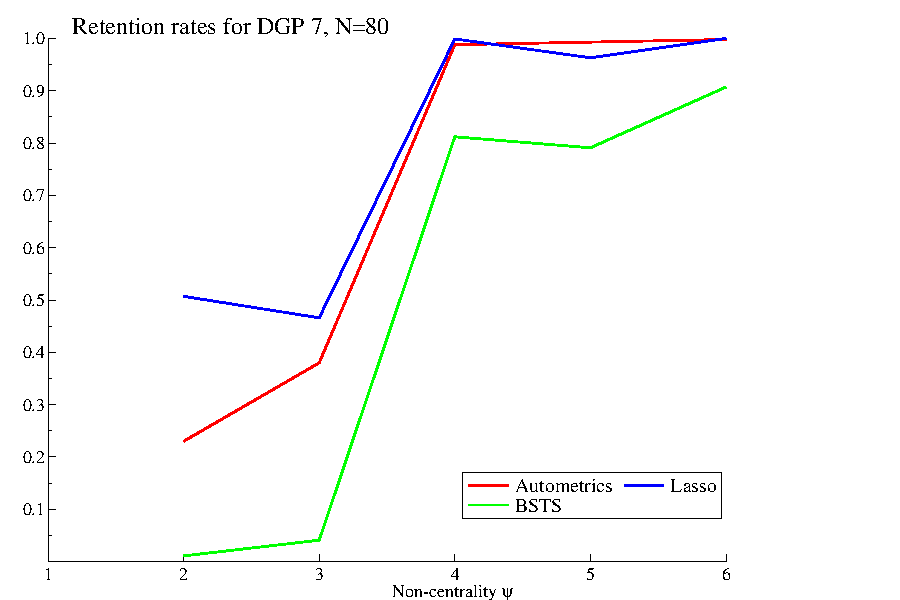
\includegraphics[scale=0.5]{RetRatesDGP7a}
\caption{Retention Rates DGP 7 \newline $N=80$}
\label{fig:RetRatesDGP7a}

\end{minipage}

\end{figure}

\begin{figure}[h]

\begin{minipage}{.5\textwidth}
\centering
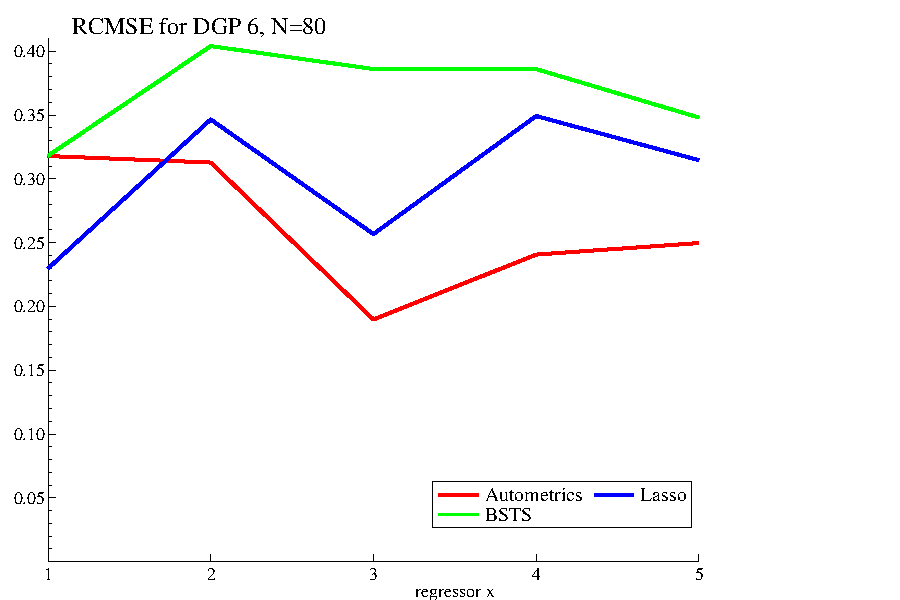
\includegraphics[scale=0.5]{RCMSE-DGP6a}
\caption{RCMSE DGP 6 \newline $N=80$}
\label{fig:CMSEDGP6a}
\end{minipage}%
\begin{minipage}{.5\textwidth}
\centering
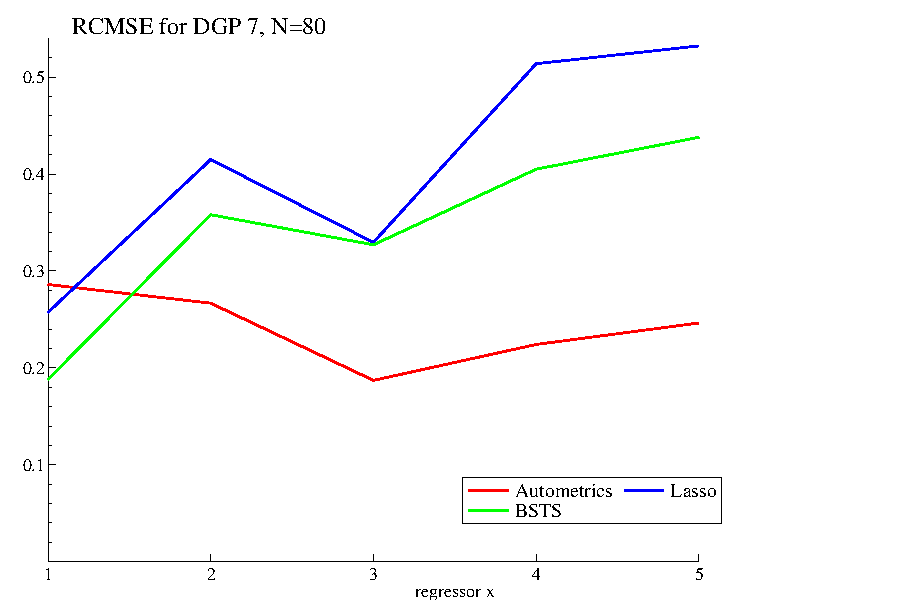
\includegraphics[scale=0.5]{RCMSE-DGP7a}
\caption{RCMSE DGP 7 \newline $N=80$}
\label{fig:CMSEDGP7a}

\end{minipage}

\end{figure}




\begin{figure}[h]

\begin{minipage}{.5\textwidth}
\centering
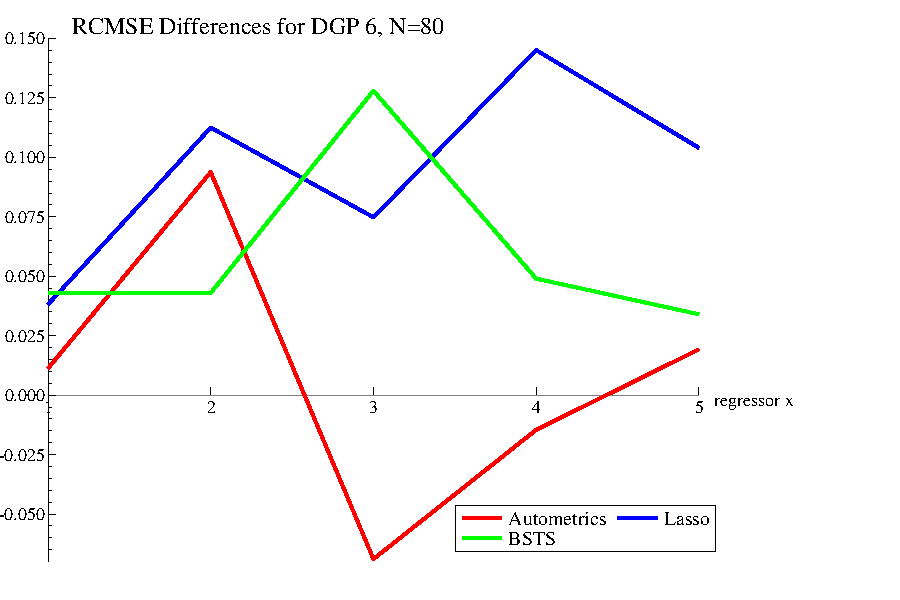
\includegraphics[scale=0.5]{RCMSEDiffDGP6a}
\caption{RCMSE differences DGP 6 \newline $N=80$}
\label{fig:CMSEDGP6a}
\end{minipage}%
\begin{minipage}{.5\textwidth}
\centering
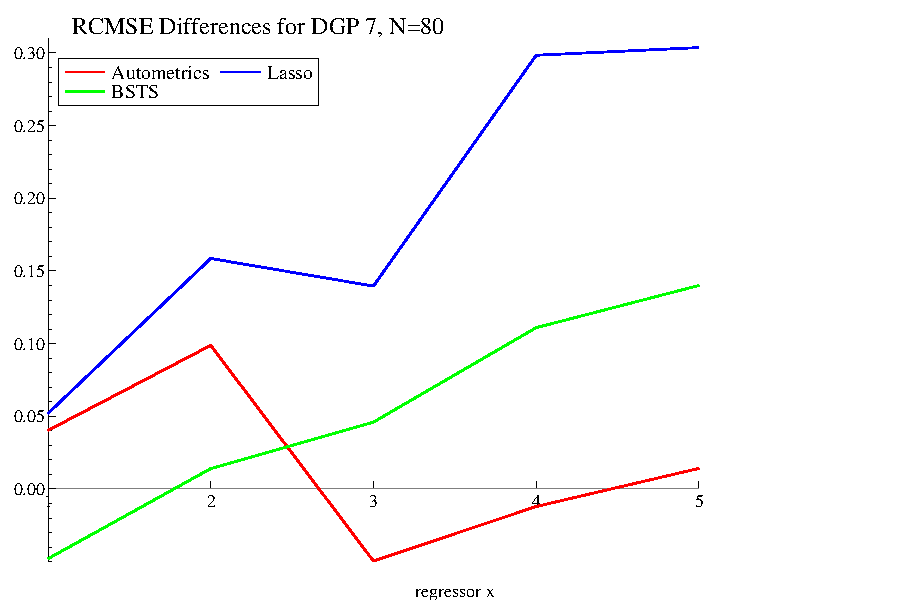
\includegraphics[scale=0.5]{RCMSEDiffDGP7a}
\caption{RCMSE differences DGP 7 \newline $N=80$}
\label{fig:CMSEDGP7a}

\end{minipage}

\end{figure}

\clearpage

First considering the results from DGP 6, the Lasso appears to be effective at identifying relevant variables but also tends to select many irrelevant variables overall, as evidenced by the high gauge. When $\psi>3$, the retention rates for all three algorithms are very high. The gauge for Autometrics is slightly higher than the significance level $\alpha$, and almost 0 for BSTS. The RCMSE are generally highest for BSTS and lowest for Autometrics. Search costs are lowest for Autometrics. 

With the DGP 7 results, the retention rates are similar to those of DGP 6 but different in a subtle and important way. Both the Lasso and BSTS struggle to pick up variables with $\psi>0$. Similarly, the Lasso struggles to estimate the parameters on variables with $\psi>0$. These difficulties are not as pronounced as in the previous set of experiments, but clear nonetheless. While the Lasso and BSTS struggle increasingly to estimate the parameter estimates as $|\psi|$ increases, Autometrics has RCMSEs which are low and consistent for all variables. 

Comparing DGP 6 and DGP 7, several important differences arise. While in theory the DGPs are very similar with almost identical properties, the results vary. The Lasso and BSTS again appear to struggle with alternating signs both in terms of how effectively they pick up relevant variables and how accurate the parameter estimates are. The measures of gauge are consistent across all algorithms in both DGP 6 and DGP 7; again BSTS with the lowest gauge near 0, the Lasso with the highest in the range of 0.13-0.18, and Autometrics in the middle with gauges slightly above the significance level.

An additional observation is that the Lasso struggled less when dealing with alternating signs and all variables correlated in this set of experiments, than it did when only the relevant regressors were correlated in the previous set of experiments. This is likely due to the fact that in this set of experiments the correlation between all variables was $\omega_{jk} = 0.8$ and in the previous set of experiments the correlation between relevant variables was $\omega_{jk} = 0.9$. 

The takeaways from this set of experiments are:
\begin{enumerate}
\item Alternating signs matter a lot for the Lasso, a reasonable amount for BSTS and a little for Autometrics. Note that negative coefficients and positive correlations are isomorphic to positive coefficients and negative correlations, so this result would also hold if it parameter signs were switched.
\item The Lasso is excellent at selecting relevant variables when all the signs are the same, but not very good at excluding irrelevant variables.
\item The gauge for Autometrics is consistently slightly above the significance level for all experiments. 
\item BSTS generally selects very sparse models, which do not include many relevant or irrelevant variables.
\end{enumerate}.

\clearpage
























 








\newpage

\section{Results Summary}

Evaluating the algorithms up until this point has focused on comparing the results from model selection conditional on a known correlation structure between the regressors. Therefore, when thinking about what the results in the previous section say about empirical model selection, the correlation structure of the variables under consideration must be taken into account. For example, if a researcher used Autometrics or the Lasso on a set of orthogonal variables, she would know that the model selected by Autometrics included $\alpha$\% of the irrelevant variables, and the model selected by the Lasso included 15-20\% of the irrelevant variables. Additionally she would know there was a 99\% chance that a variable with a signal-to-noise ratio of 4 was included in the selected model. These statements rely on orthogonality however, and given that the world is dynamic, full of relationships and extremely interdependent, orthogonal results on their own are of limited use. Because a researcher never knows the true DGP, she cannot possibly know what the true correlation structure is. Thus, to truly be able to interpret and say something meaningful about the effectiveness of model selection empirically, it is vital to understand how different `states of nature' influence the results. Since a researcher can never know the true DGP and therefore cannot qualify results in this manner, ideally model selection results should not depend on the correlation structure.

A desirable property of model selection would be for a variable with a given `significance', which can be measured by its non-centrality, to be selected at the same level regardless of the properties of the other variables in the GUM. It is for this reason that in each of the three sets of experiments, $\beta_{1},...,\beta_{5}$ were chosen so that non-centralities are the same and retention rates and RCMSEs are comparable across experiments. Looking at how results vary across the three different correlation structures is therefore a straightforward way to analyze how orthogonality or otherwise influences results across values of $\psi$. Table \ref{tab:SummaryPositive} shows a summary of the results for DGP 3, DGP 4, and DGP 6 for $N=80$. Similarly, Table \ref{tab:SummaryAlt} shows the results for DGPs with alternating signs. Note that results from alternating signs when the regressors are orthogonal are largely the same as when the signs are all the same, and were not reported earlier. 

% Table generated by Excel2LaTeX from sheet 'Allpositive-noformulas'

\begin{landscape}

\begin{table}[htbp]
  \centering

    \begin{tabular}{r|rrr|rrr|rrr}
  & \multicolumn{3}{c|}{\textbf{Autometrics}}  & \multicolumn{3}{c|}{\textbf{Lasso}}                                                   & \multicolumn{3}{c}{\textbf{BSTS}}                        \\ \hline
$\psi$ & Orthogonal & Some Corr & All Corr & Orthogonal & Some Corr & All Corr & Orthogonal & Some Corr                & All Corr \\ \hline
    2     & 0.216 & 0.333 & 0.262 & 0.552 & 0.977 & 0.766 & 0.003 & 0.179 & 0.116 \\
    3     & 0.414 & 0.568 & 0.439 & 0.869 & 0.990  & 0.778 & 0.136 & 0.340  & 0.251 \\
    4     & 0.948 & 0.988 & 0.985 & 0.974 & 1.000     & 1.000     & 0.325 & 0.949 & 0.923 \\
    5     & 0.989 & 0.998 & 0.996 & 0.995 & 1.000     & 1.000     & 0.562 & 0.993 & 0.984 \\
    6     & 0.995 & 0.998 & 0.996 & 0.996 & 1.000     & 1.000     & 0.781 & 0.991 & 0.99 \\
   \hline
    Potency & 0.712 & 0.777 & 0.736 & 0.877 & 0.993 & 0.909 & 0.361 & 0.690 & 0.653 \\
    Gauge & 0.018 & 0.014 & 0.016 & 0.179 & 0.108 & 0.182 & 0.001 & 0.000 & 0.004 \\


 
    \end{tabular}%
 
    \caption{Retention rate, potency and gauge summary results for all positive $\psi$}
     \label{tab:SummaryPositive}%
\end{table}%

% Table generated by Excel2LaTeX from sheet 'Alternating-noformulas'
\begin{table}[htbp]
  \centering

    \begin{tabular}{r|rrr|rrr|rrr}
  & \multicolumn{3}{c|}{\textbf{Autometrics}}  & \multicolumn{3}{c|}{\textbf{Lasso}}                                                   & \multicolumn{3}{c}{\textbf{BSTS}}                        \\ \hline
$\psi$ & Orthogonal & Some Corr & All Corr & Orthogonal & Some Corr & All Corr & Orthogonal & Some Corr                & All Corr \\ \hline

    -2    & 0.240  & 0.255 & 0.230  & 0.608 & 0.065 & 0.507 & 0.007 & 0.022 & 0.011 \\
    3     & 0.476 & 0.355 & 0.380  & 0.74  & 0.013 & 0.466 & 0.043 & 0.056 & 0.041 \\
    -4    & 0.928 & 0.981 & 0.988 & 0.981 & 0.984 & 0.999 & 0.349 & 0.798 & 0.812 \\
    5     & 0.993 & 0.996 & 0.993 & 1.000     & 0.095 & 0.963 & 0.943 & 0.827 & 0.791 \\
    -6    & 0.996 & 0.994 & 0.998 & 0.998 & 0.988 & 1.000     & 0.792 & 0.951 & 0.907 \\
    \hline
    Potency & 0.727 & 0.716 & 0.718 & 0.865 & 0.429 & 0.787 & 0.427 & 0.531 & 0.512 \\
    Gauge & 0.018 & 0.014 & 0.014 & 0.176 & 0.088 & 0.154 & 0.000 & 0.000 & 0.001 \\

    \end{tabular}%
  
    \caption{Retention rate, potency and gauge summary results for alternating $\psi$}
    \label{tab:SummaryAlt}%
\end{table}%

\end{landscape}

These two tables contain many interesting insights. The results for Autometrics do not vary significantly across the different correlation structures, both when $\psi_{k}>0,\forall k$ and when the signs of $\psi$ alternate. As $|\psi|$ increases, correlation matters less and results converge to 1. The gauge is also consistent across correlation structures, fluctuating between 0.014 and 0.018.  The Lasso, on the other hand, exhibits a very different story. While when $\psi_{k}>0, \forall k$, and $\psi>3$ the retention rates are consistent across the correlation structures, this is not the case when the signs are alternating. In fact, in the case of alternating signs, the Lasso picks up variable $x_{k}$ with $\psi_{k}=3$, 74\% of the time when the regressors are orthogonal, compared to 1\% of the time when there is correlation between the relevant regressors, and 46\% of the time when there is correlation between all regressors. The gauge in the Lasso experiments is also remarkably varied, ranging between 0.09 and 0.18. These discrepancies and their implications are substantial. The same is true but to a lesser extent for BSTS where there is notable variation in retention rates across the three correlation structures, especially when $|\psi|<4$. The gauge for BSTS, on the other hand, has almost no variation.

Figure \ref{fig:GaugePot} provides an interesting visual representation of the results in the previous two tables. The potency and gauge are plotted against each other for both $N=80$ and $N=120$, meaning that a total of twelve experiments are graphed. The experiments graphed have properties such that one would expect MC results to be similar. The ideal algorithm would have all of its points bunched in the upper left corner of the graph. As can be easily seen, the Lasso and BSTS points are decidedly not in the upper left quadrant. In fact, the Lasso has points all over the graph. While BSTS consistently achieves low gauges, it fares poorly when it comes to potency. Autometrics points are grouped together closely. While it may not always have as high a potency as the Lasso, or as low a gauge as BSTS, it does reasonably well in both and perhaps more importantly is consistent in the sense that the correlation structure of the regressors has no bearing on the results. 

\begin{figure}[h]


\centering
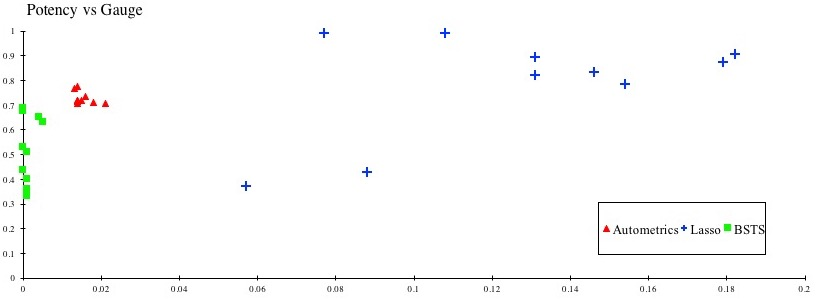
\includegraphics[scale=.5]{GPGraph}
\caption{Scatter plot of potency vs. gauge across all experiments}
\label{fig:GaugePot}


\end{figure}


\subsection{What do the Monte Carlo simulation results say about empirical model selection?}

As should be clear by now, model selection is difficult to evaluate empirically; it is impossible to judge how `good' a selected model is because it is impossible to know what to be judging against. This is why the results from MC simulations are so important and useful, and in particular why analyzing what happens when correlation structures change is vital. Because a modeller can never know what the properties of the relevant variables are, to draw valuable insight from selected models it is key that model selection not be reliant on what those properties are. With this in mind, the results in this study imply that a modeller performing model selection using the three algorithms can assume the following:

\textbf{Autometrics}
\begin{enumerate}
\item There are slightly higher than 100($\alpha$)\% of the total number of irrelevant variables included in the selected model. 
\item The probability that a variable with `significance', in signal-to-noise terms of $\psi$ has been selected can be approximated by the theoretical retention probability formula.
\item The costs of inference, or equivalently the parameter estimate accuracy, does not vary according to how `significant' a variable is. (Bias correction has not been employed here, but studies show that this a costless way of improving parameter accuracy. See Hendry and Krolzig (2005))
\item The costs of search for using Autometrics are minimal and sometimes even negative. That is, a researcher will `lose' almost nothing employing Autometrics, but stands to gain considerably.
\end{enumerate}

\textbf{Lasso}
\begin{enumerate}
\item There can be anywhere in the range of 8-20\% of the total number of irrelevant variables included in the selected model. When $N=120$, this implies keeping up to 24 irrelevant variables, compared to 6 relevant variables.
\item If all the important variables in the model happen to be relevant to the dependent variables in the same `direction' (i.e. all matter in either a positive or negative way for the dependent variable), then the Lasso will identify and select them with a high probability. In particular, a variable with a signal-to-noise ratio of $\psi>3$ has over a 97\% change of being selected.
\item The probability of selecting a relevant variable with a lower signal-to-noise ratio varies according to how correlated it is with the other variables in the model. For example the probability of selecting a variable with a signal-to-noise ratio of $\psi=2$ can be anywhere in the range of 55-98\%. 
\item Parameter estimates become increasingly inaccurate the more `significant' a variable is.
\end{enumerate}

\textbf{BSTS}
\begin{enumerate}
\item There are almost no irrelevant variables (around 0.1\%) included in the selected model.
\item This sparsity has an impact on the inability to keep relevant variables.
\item BSTS is affected by the correlation structure of the regressors, and the signs of the coefficients.
% \item another? 
\end{enumerate}